\documentclass[]{article}
\usepackage{lmodern}
\usepackage{amssymb,amsmath}
\usepackage{ifxetex,ifluatex}
\usepackage{fixltx2e} % provides \textsubscript
\ifnum 0\ifxetex 1\fi\ifluatex 1\fi=0 % if pdftex
  \usepackage[T1]{fontenc}
  \usepackage[utf8]{inputenc}
\else % if luatex or xelatex
  \ifxetex
    \usepackage{mathspec}
  \else
    \usepackage{fontspec}
  \fi
  \defaultfontfeatures{Ligatures=TeX,Scale=MatchLowercase}
\fi
% use upquote if available, for straight quotes in verbatim environments
\IfFileExists{upquote.sty}{\usepackage{upquote}}{}
% use microtype if available
\IfFileExists{microtype.sty}{%
\usepackage{microtype}
\UseMicrotypeSet[protrusion]{basicmath} % disable protrusion for tt fonts
}{}
\usepackage[margin=1in]{geometry}
\usepackage{hyperref}
\hypersetup{unicode=true,
            pdftitle={Simulation of PCB with resampling},
            pdfauthor={Xuelong Wang},
            pdfborder={0 0 0},
            breaklinks=true}
\urlstyle{same}  % don't use monospace font for urls
\usepackage{graphicx,grffile}
\makeatletter
\def\maxwidth{\ifdim\Gin@nat@width>\linewidth\linewidth\else\Gin@nat@width\fi}
\def\maxheight{\ifdim\Gin@nat@height>\textheight\textheight\else\Gin@nat@height\fi}
\makeatother
% Scale images if necessary, so that they will not overflow the page
% margins by default, and it is still possible to overwrite the defaults
% using explicit options in \includegraphics[width, height, ...]{}
\setkeys{Gin}{width=\maxwidth,height=\maxheight,keepaspectratio}
\IfFileExists{parskip.sty}{%
\usepackage{parskip}
}{% else
\setlength{\parindent}{0pt}
\setlength{\parskip}{6pt plus 2pt minus 1pt}
}
\setlength{\emergencystretch}{3em}  % prevent overfull lines
\providecommand{\tightlist}{%
  \setlength{\itemsep}{0pt}\setlength{\parskip}{0pt}}
\setcounter{secnumdepth}{5}
% Redefines (sub)paragraphs to behave more like sections
\ifx\paragraph\undefined\else
\let\oldparagraph\paragraph
\renewcommand{\paragraph}[1]{\oldparagraph{#1}\mbox{}}
\fi
\ifx\subparagraph\undefined\else
\let\oldsubparagraph\subparagraph
\renewcommand{\subparagraph}[1]{\oldsubparagraph{#1}\mbox{}}
\fi

%%% Use protect on footnotes to avoid problems with footnotes in titles
\let\rmarkdownfootnote\footnote%
\def\footnote{\protect\rmarkdownfootnote}

%%% Change title format to be more compact
\usepackage{titling}

% Create subtitle command for use in maketitle
\newcommand{\subtitle}[1]{
  \posttitle{
    \begin{center}\large#1\end{center}
    }
}

\setlength{\droptitle}{-2em}

  \title{Simulation of PCB with resampling}
    \pretitle{\vspace{\droptitle}\centering\huge}
  \posttitle{\par}
    \author{Xuelong Wang}
    \preauthor{\centering\large\emph}
  \postauthor{\par}
      \predate{\centering\large\emph}
  \postdate{\par}
    \date{2018-11-16}

\usepackage{float,amsmath, bbm, siunitx, bm}
\floatplacement{figure}{H}
\newcommand{\indep}{\rotatebox[origin=c]{90}{$\models$}}

\begin{document}
\maketitle

{
\setcounter{tocdepth}{2}
\tableofcontents
}
\section{Motivation}\label{motivation}

Based on the simulation studies, we found the proposed method could work
well even if the covariates' distributions are correlated and long tail.
More specifically, the proposed method can estimate the main and
interactive effect's variance without much bias. Thus, we have some
reason to believe that the proposed method could also work well on the
PCB data.

We want to conduct the previous simulation studies on PCB data. However,
there is a issue to be solved. One of the assumptions of GCTA method is
that the covariates are random variables. Thus, the covariates \(X\) are
randomly sampled for each iteration during the simulation procedure. But
it cannot be available for PCB data, because we only have one set of
data with 1000 observations.

\section{Re-sampling procedure}\label{re-sampling-procedure}

To solve the problem mentioned above, we could used the resampling PCB's
observations without replacement to mimic the randomization of the
covariates. Although those re-sampled data is not the true random
variable, it more or less can give as an idea that how well the proposed
method can work on the PCB data.

\subsection{Bootstrap VS Resampling}\label{bootstrap-vs-resampling}

Resampling method can keep the observed covariance structure of the PCB
data. However, since the bootstrap using sampling with replacement, it
cannot keep the original structure.

\[
  X = \begin{bmatrix}   
        x_1\\
        x_2\\
        x_3
      \end{bmatrix},
  \Sigma = \begin{bmatrix}   
        \sigma_{11} ~ \sigma_{12} ~ \sigma_{13}\\
        \sigma_{21} ~ \sigma_{22} ~ \sigma_{23}\\
        \sigma_{31} ~ \sigma_{32} ~ \sigma_{33}\\
      \end{bmatrix}
\]

\[
  X_{resample} = \begin{bmatrix}   
        x_1\\
        x_2\\
      \end{bmatrix},
  \Sigma = \begin{bmatrix}   
        \sigma_{11} ~ \sigma_{12}\\
        \sigma_{21} ~ \sigma_{22}
      \end{bmatrix}
\]

\[
  X_{bootstrap} = \begin{bmatrix}   
        x_1\\
        x_2\\
        x_2
      \end{bmatrix},
  \Sigma = \begin{bmatrix}   
        \sigma_{11} ~ \sigma_{12} ~ \sigma_{12}\\
        \sigma_{21} ~ \sigma_{22} ~ \sigma_{22}\\
        \sigma_{21} ~ \sigma_{22} ~ \sigma_{22}\\
      \end{bmatrix}
\]

\subsection{re-sample size}\label{re-sample-size}

We need to find an appropriate sample size which is not too large to
reduce the randomization or too sample to increase the estimations
variation.

\[
  m = p * n, \text{ where $p = (0.6 - 0.9)$}
\]

\section{Simulation result}\label{simulation-result}

\subsection{Total effect estimation}\label{total-effect-estimation}

\begin{figure}
\centering
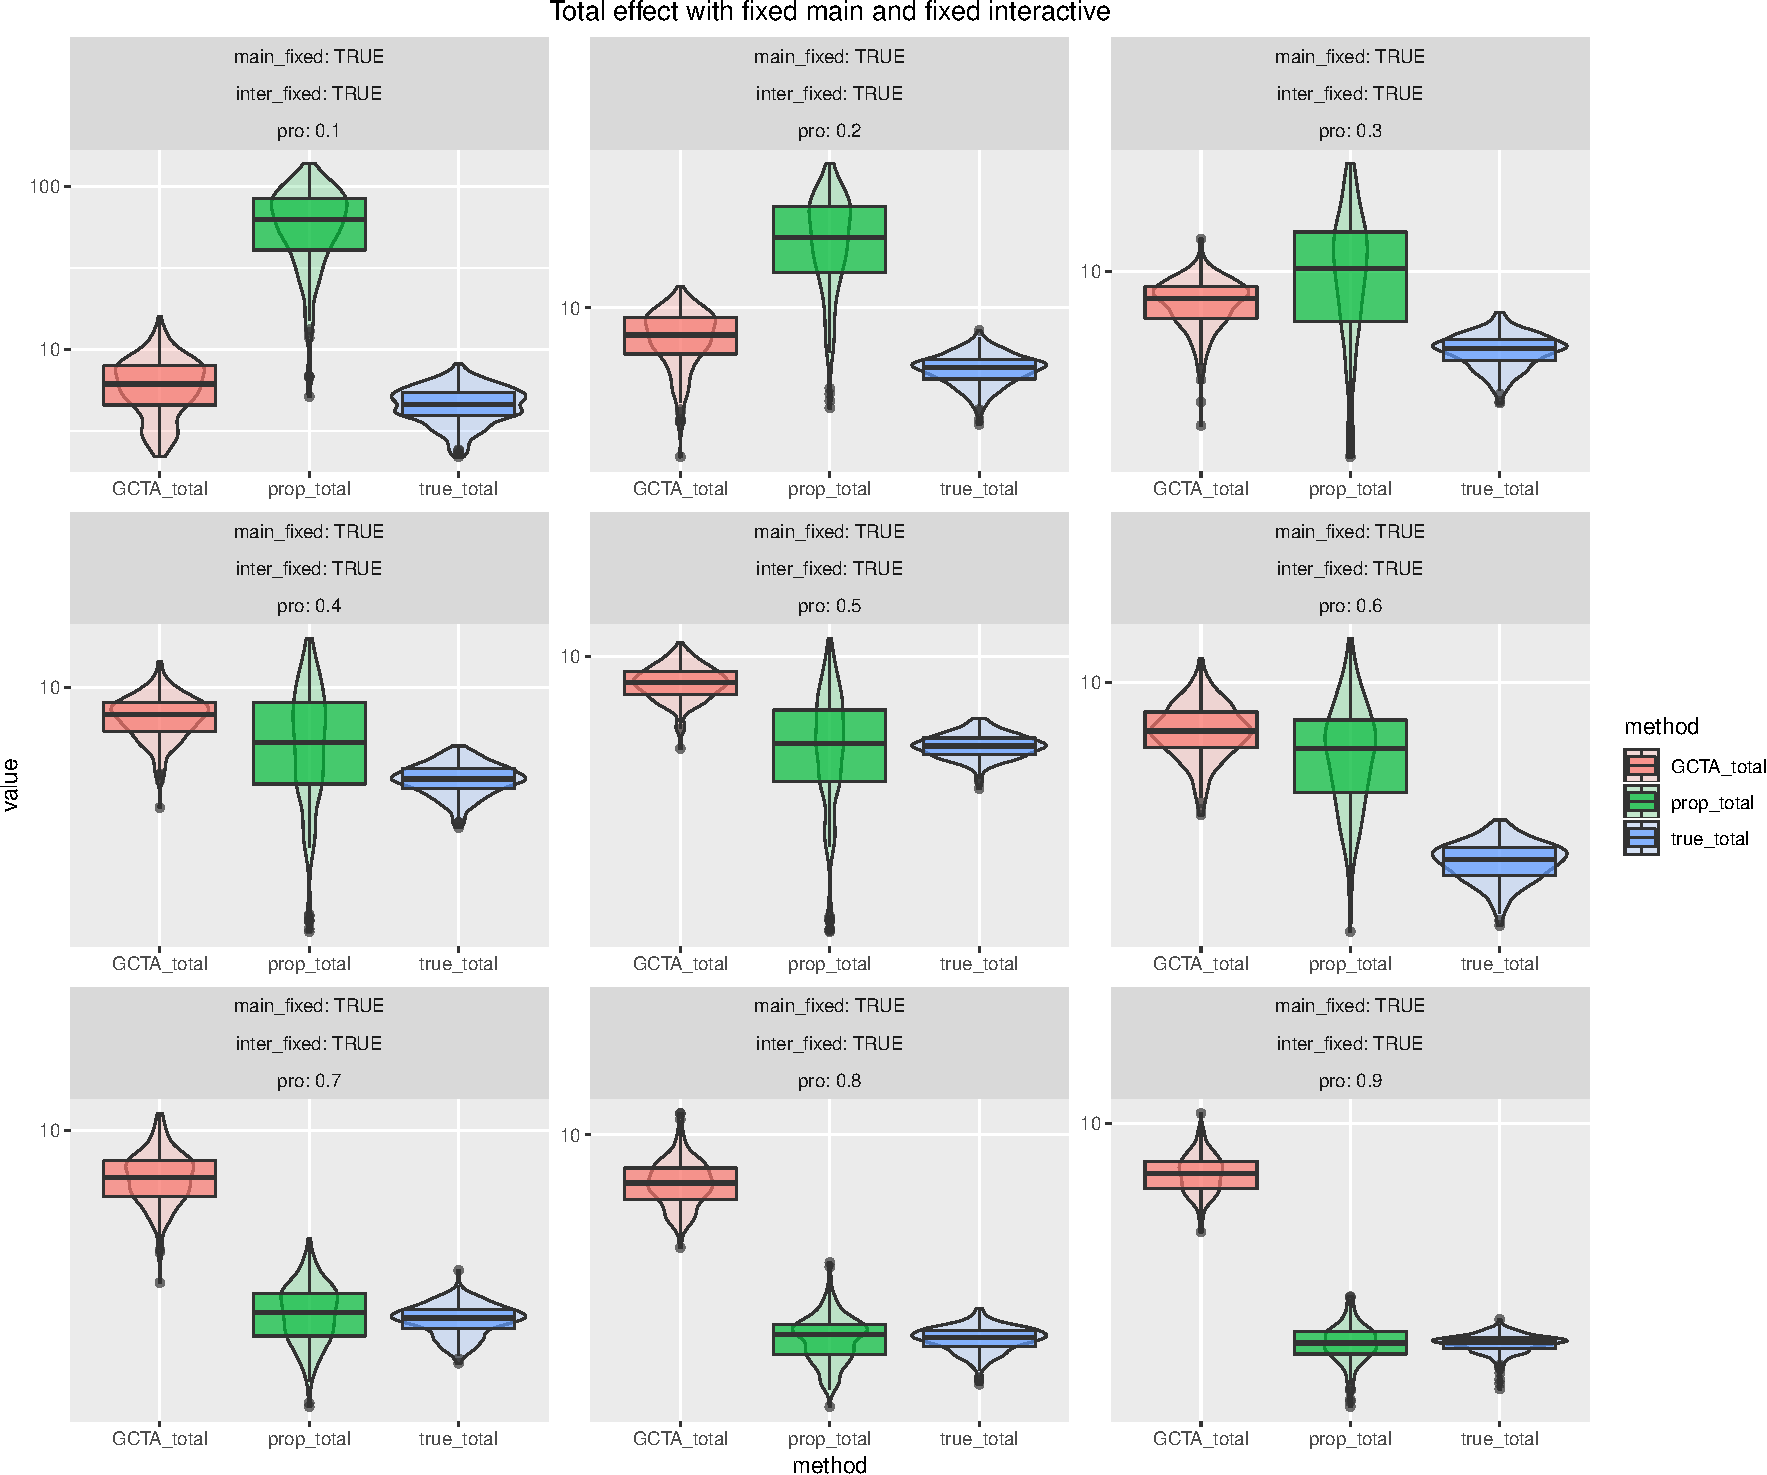
\includegraphics{Simulation_report_files/figure-latex/Total effect fixed fixed-1.pdf}
\caption{Total effect estimation with fixed main and fixed interaction}
\end{figure}

\begin{figure}
\centering
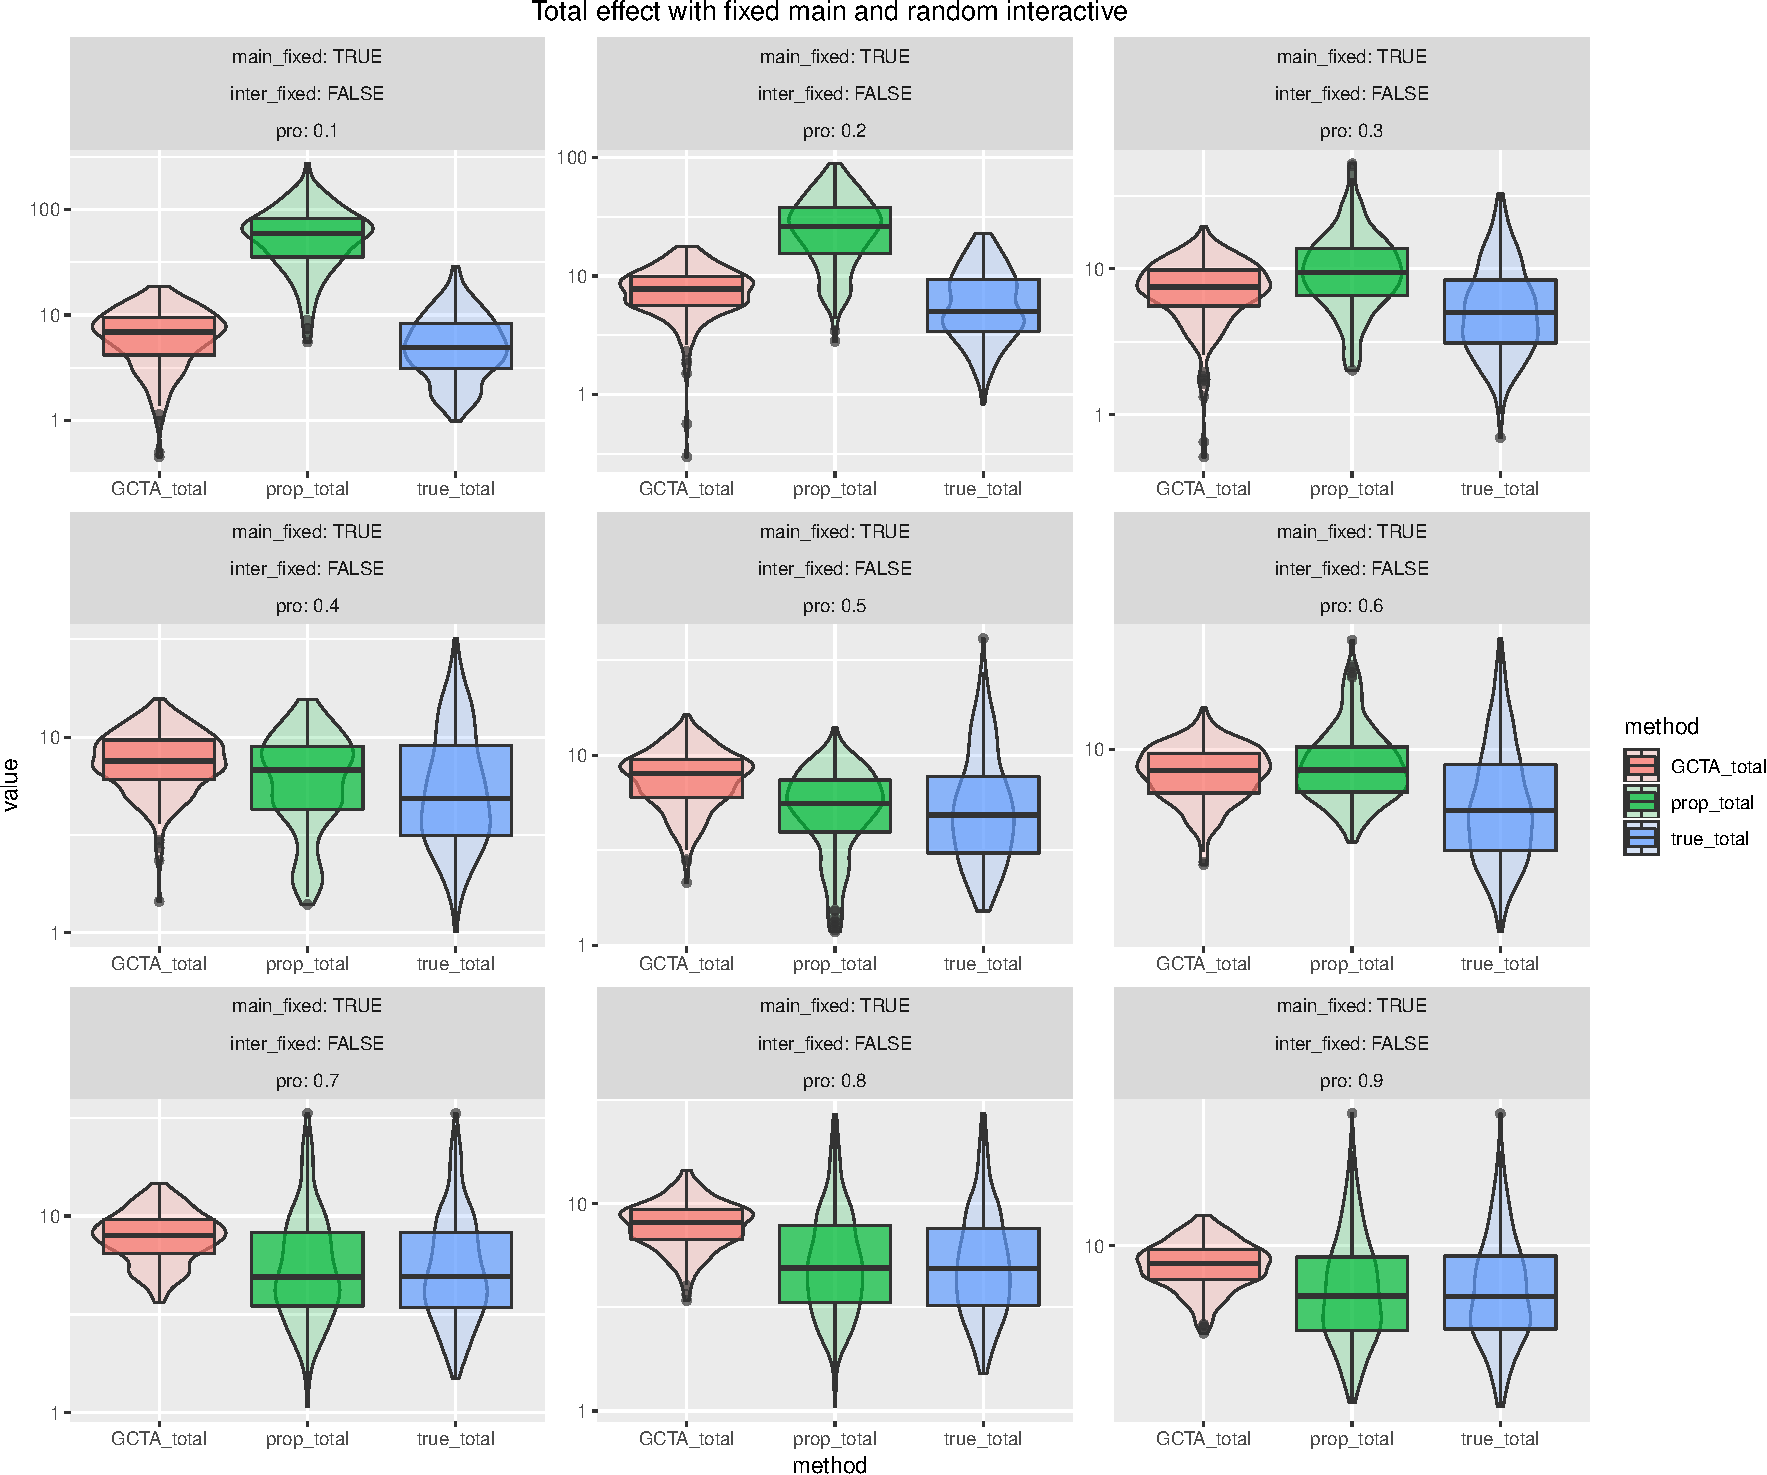
\includegraphics{Simulation_report_files/figure-latex/Total effect fixed random-1.pdf}
\caption{Total effect estimation with fixed main and random interaction}
\end{figure}

\begin{figure}
\centering
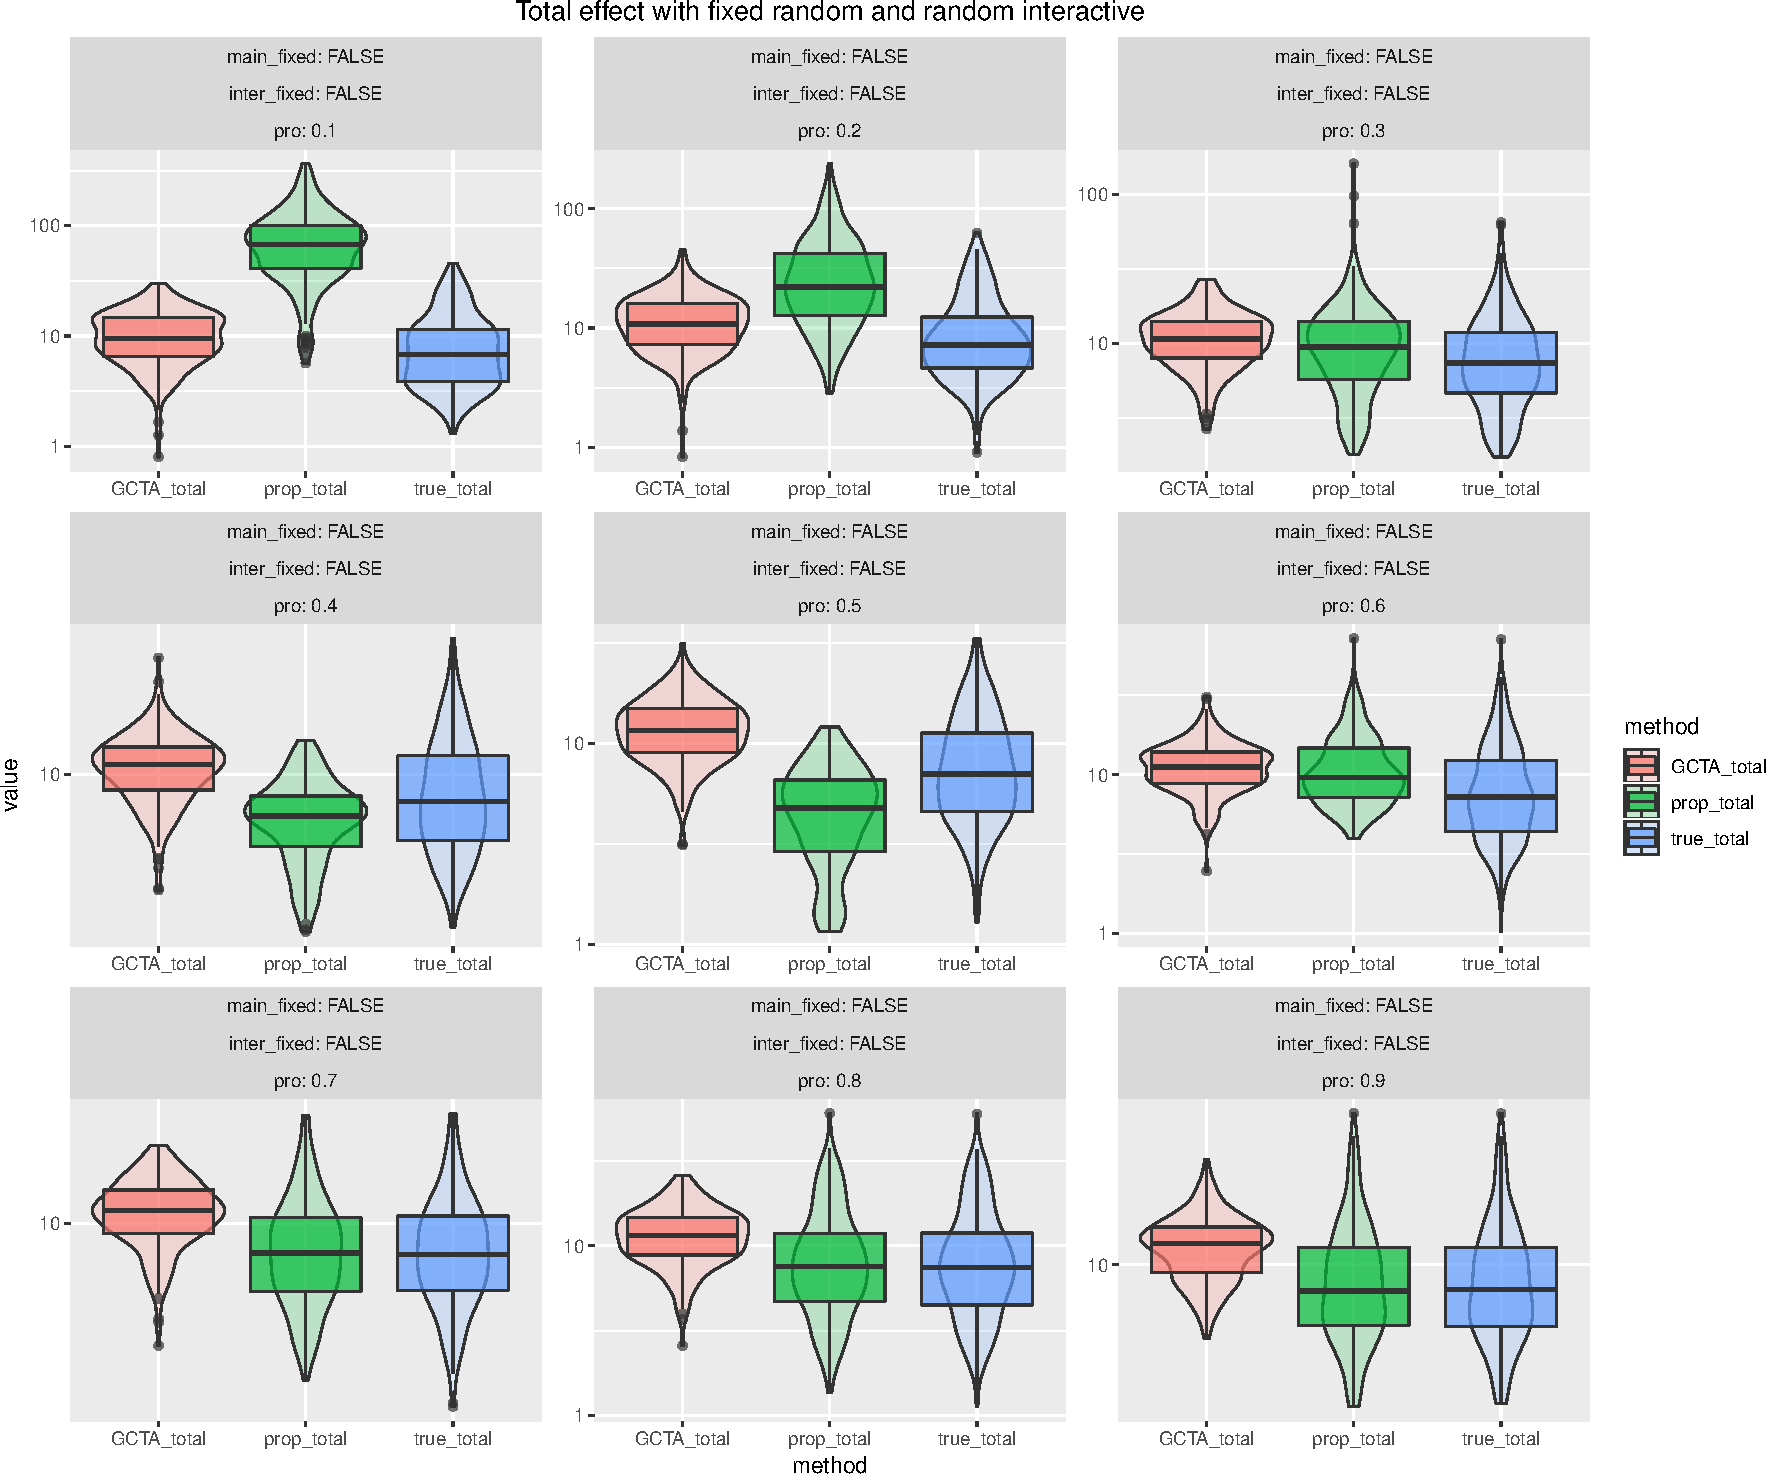
\includegraphics{Simulation_report_files/figure-latex/Total effect random random-1.pdf}
\caption{Total effect estimation with random main and random
interaction}
\end{figure}

\newpage

\subsection{Total effect estimation with p =
6}\label{total-effect-estimation-with-p-6}

\begin{figure}
\centering
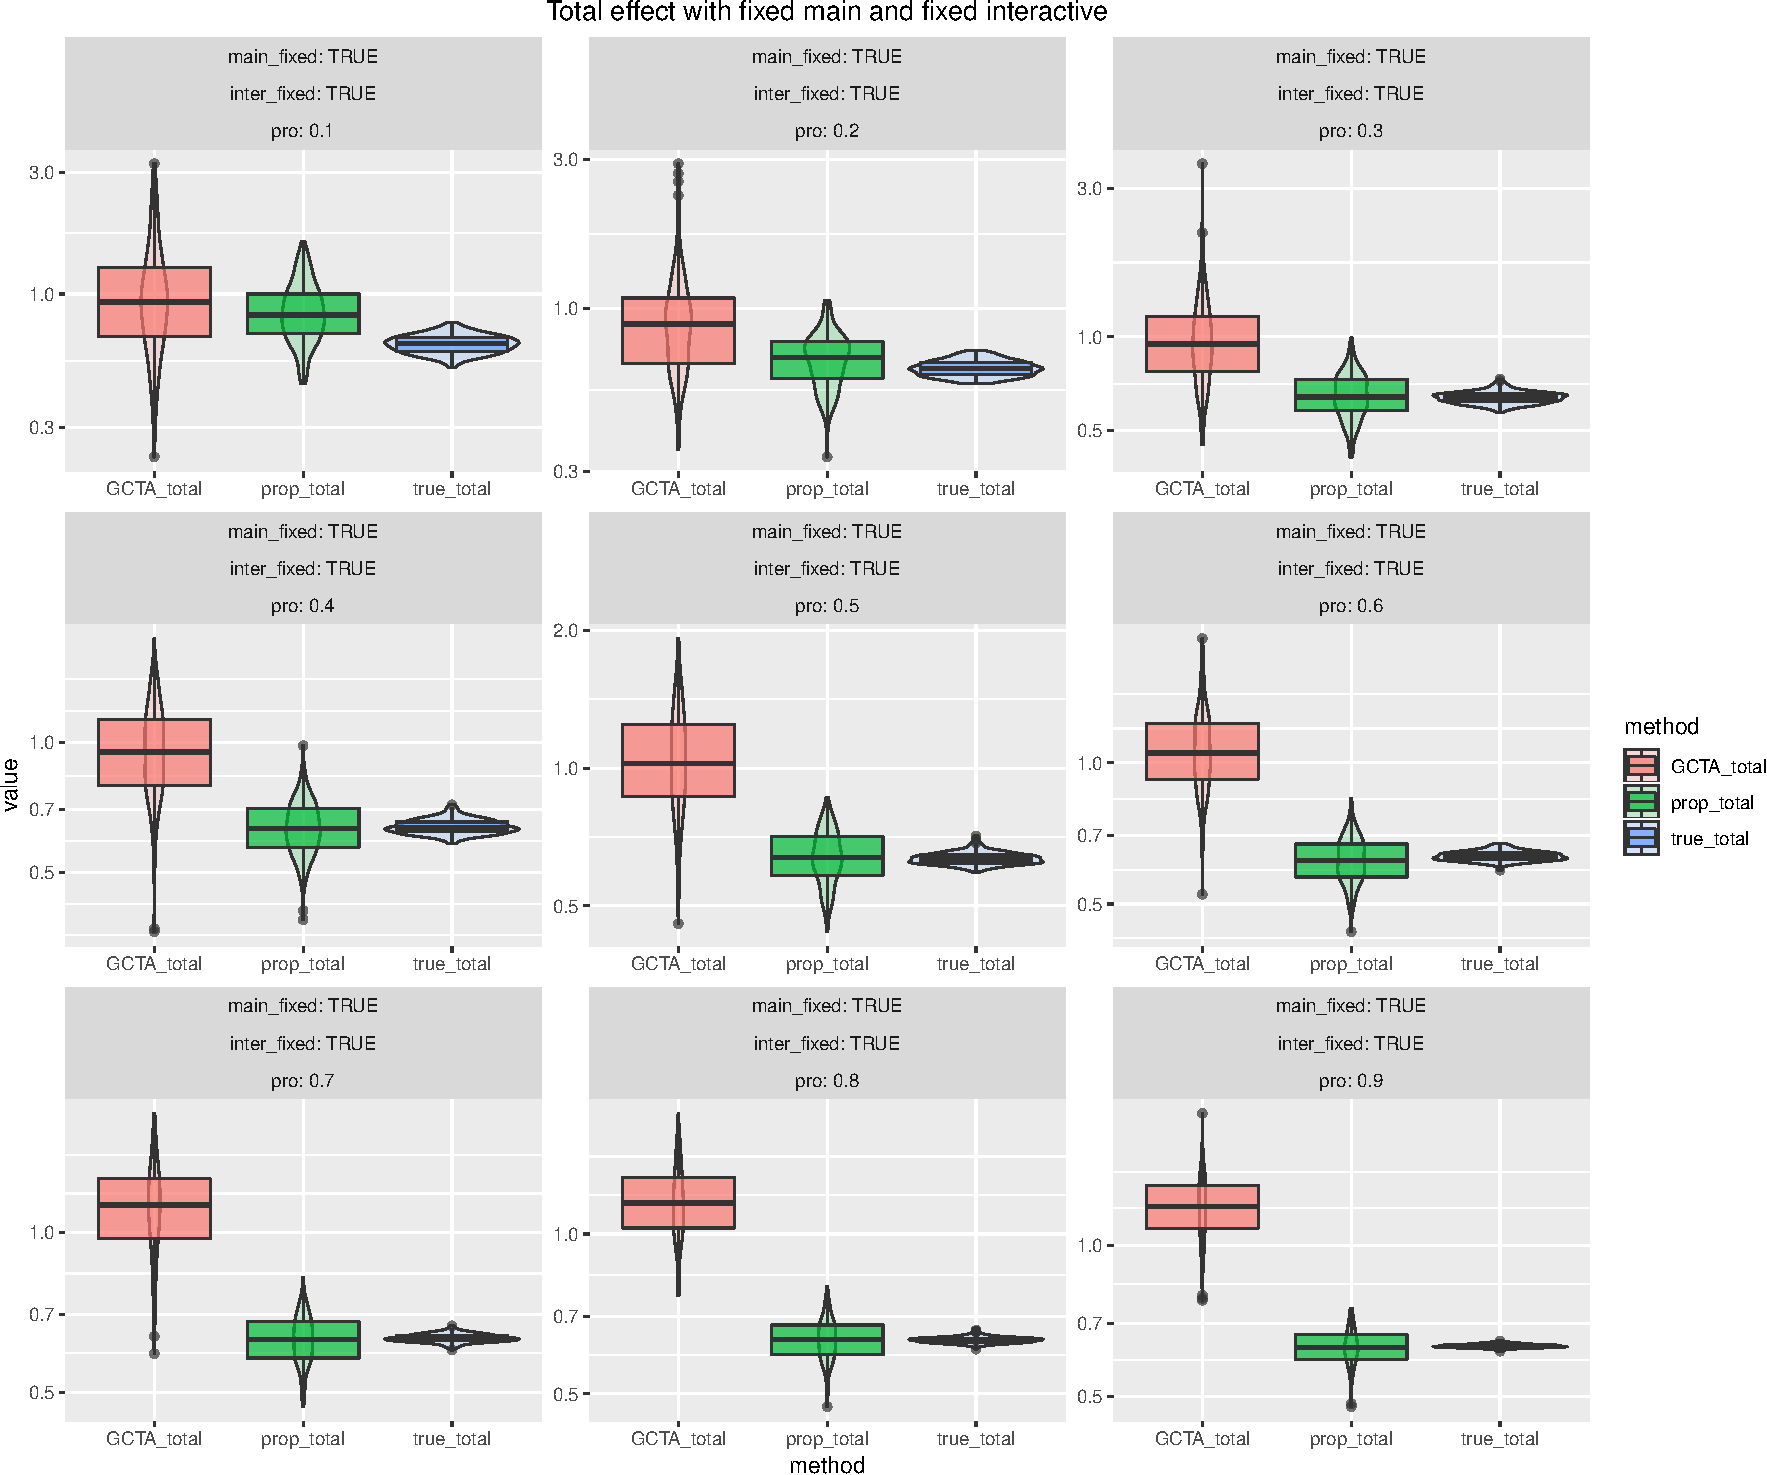
\includegraphics{Simulation_report_files/figure-latex/Total effect fixed fixed 6-1.pdf}
\caption{Total effect estimation with fixed main and fixed interaction}
\end{figure}

\begin{figure}
\centering
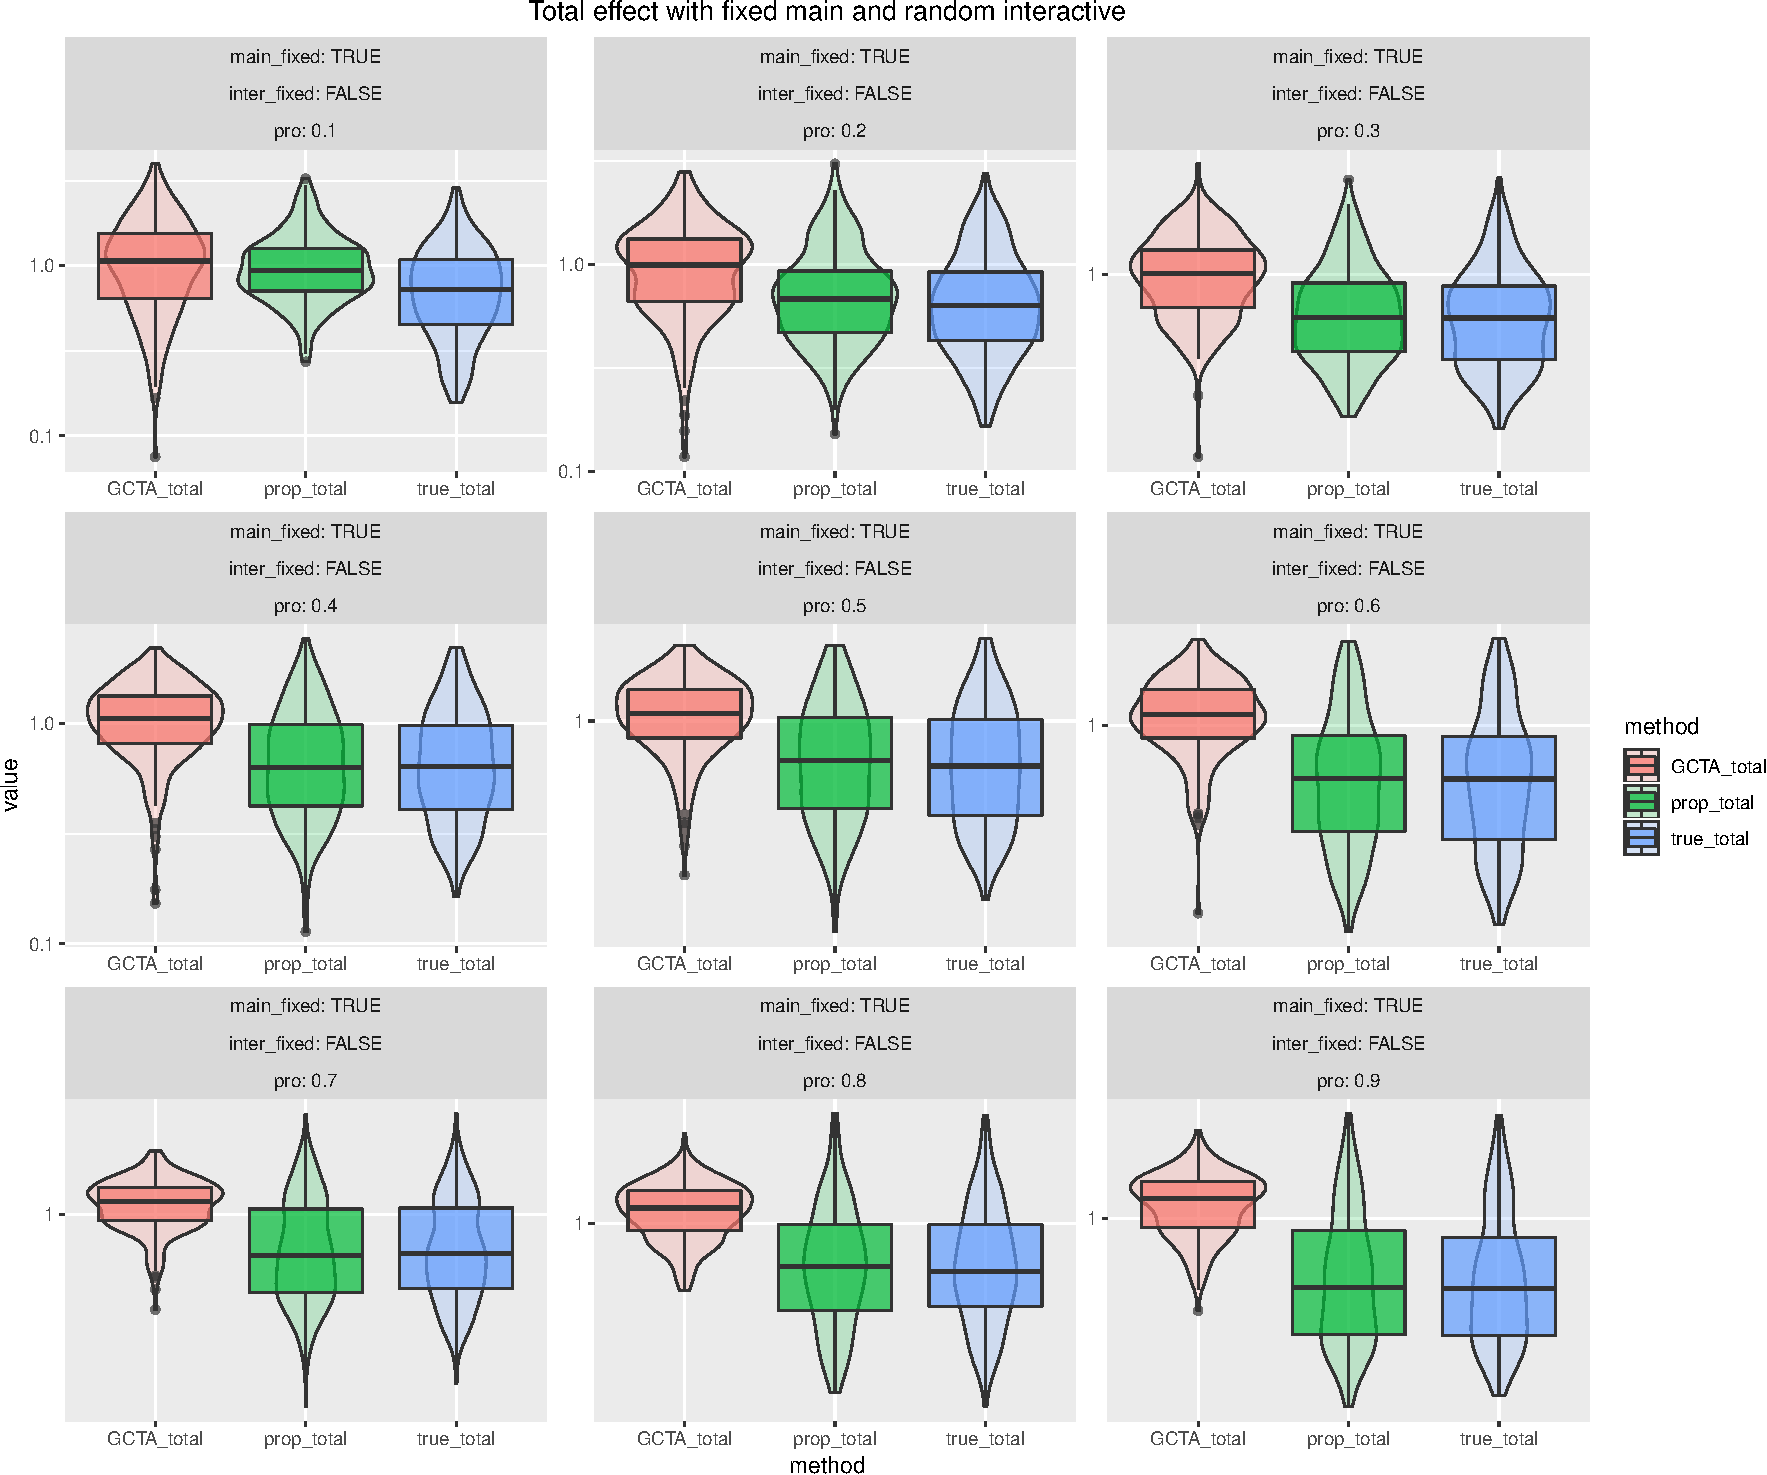
\includegraphics{Simulation_report_files/figure-latex/Total effect fixed random 6-1.pdf}
\caption{Total effect estimation with fixed main and random interaction}
\end{figure}

\begin{figure}
\centering
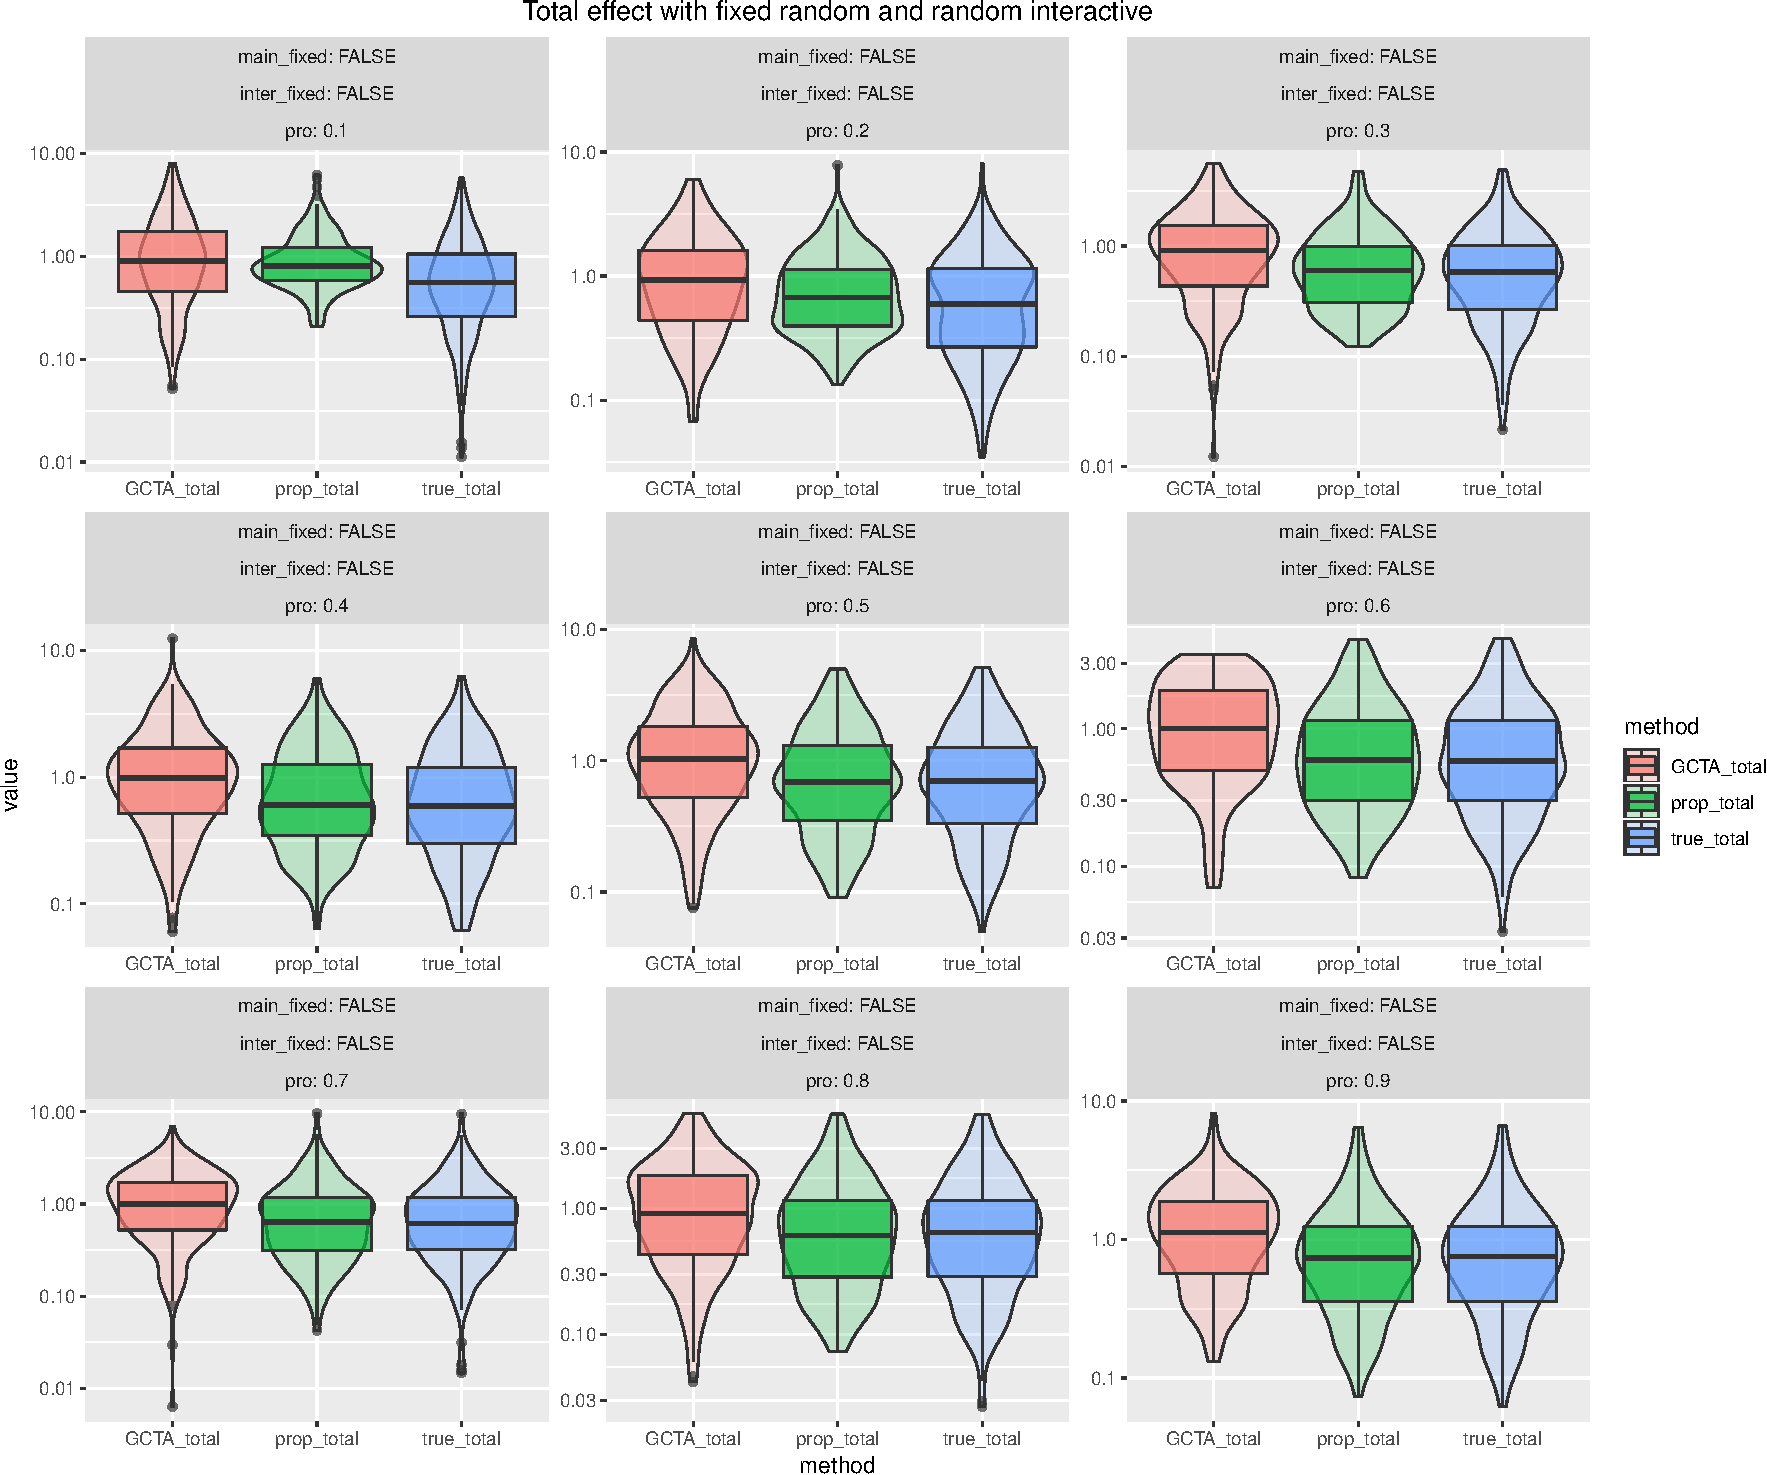
\includegraphics{Simulation_report_files/figure-latex/Total effect random random 6-1.pdf}
\caption{Total effect estimation with random main and random
interaction}
\end{figure}

\newpage

\subsection{Total effect estimation with p = 33 combined PCB data from
99 to
13}\label{total-effect-estimation-with-p-33-combined-pcb-data-from-99-to-13}

\begin{figure}
\centering
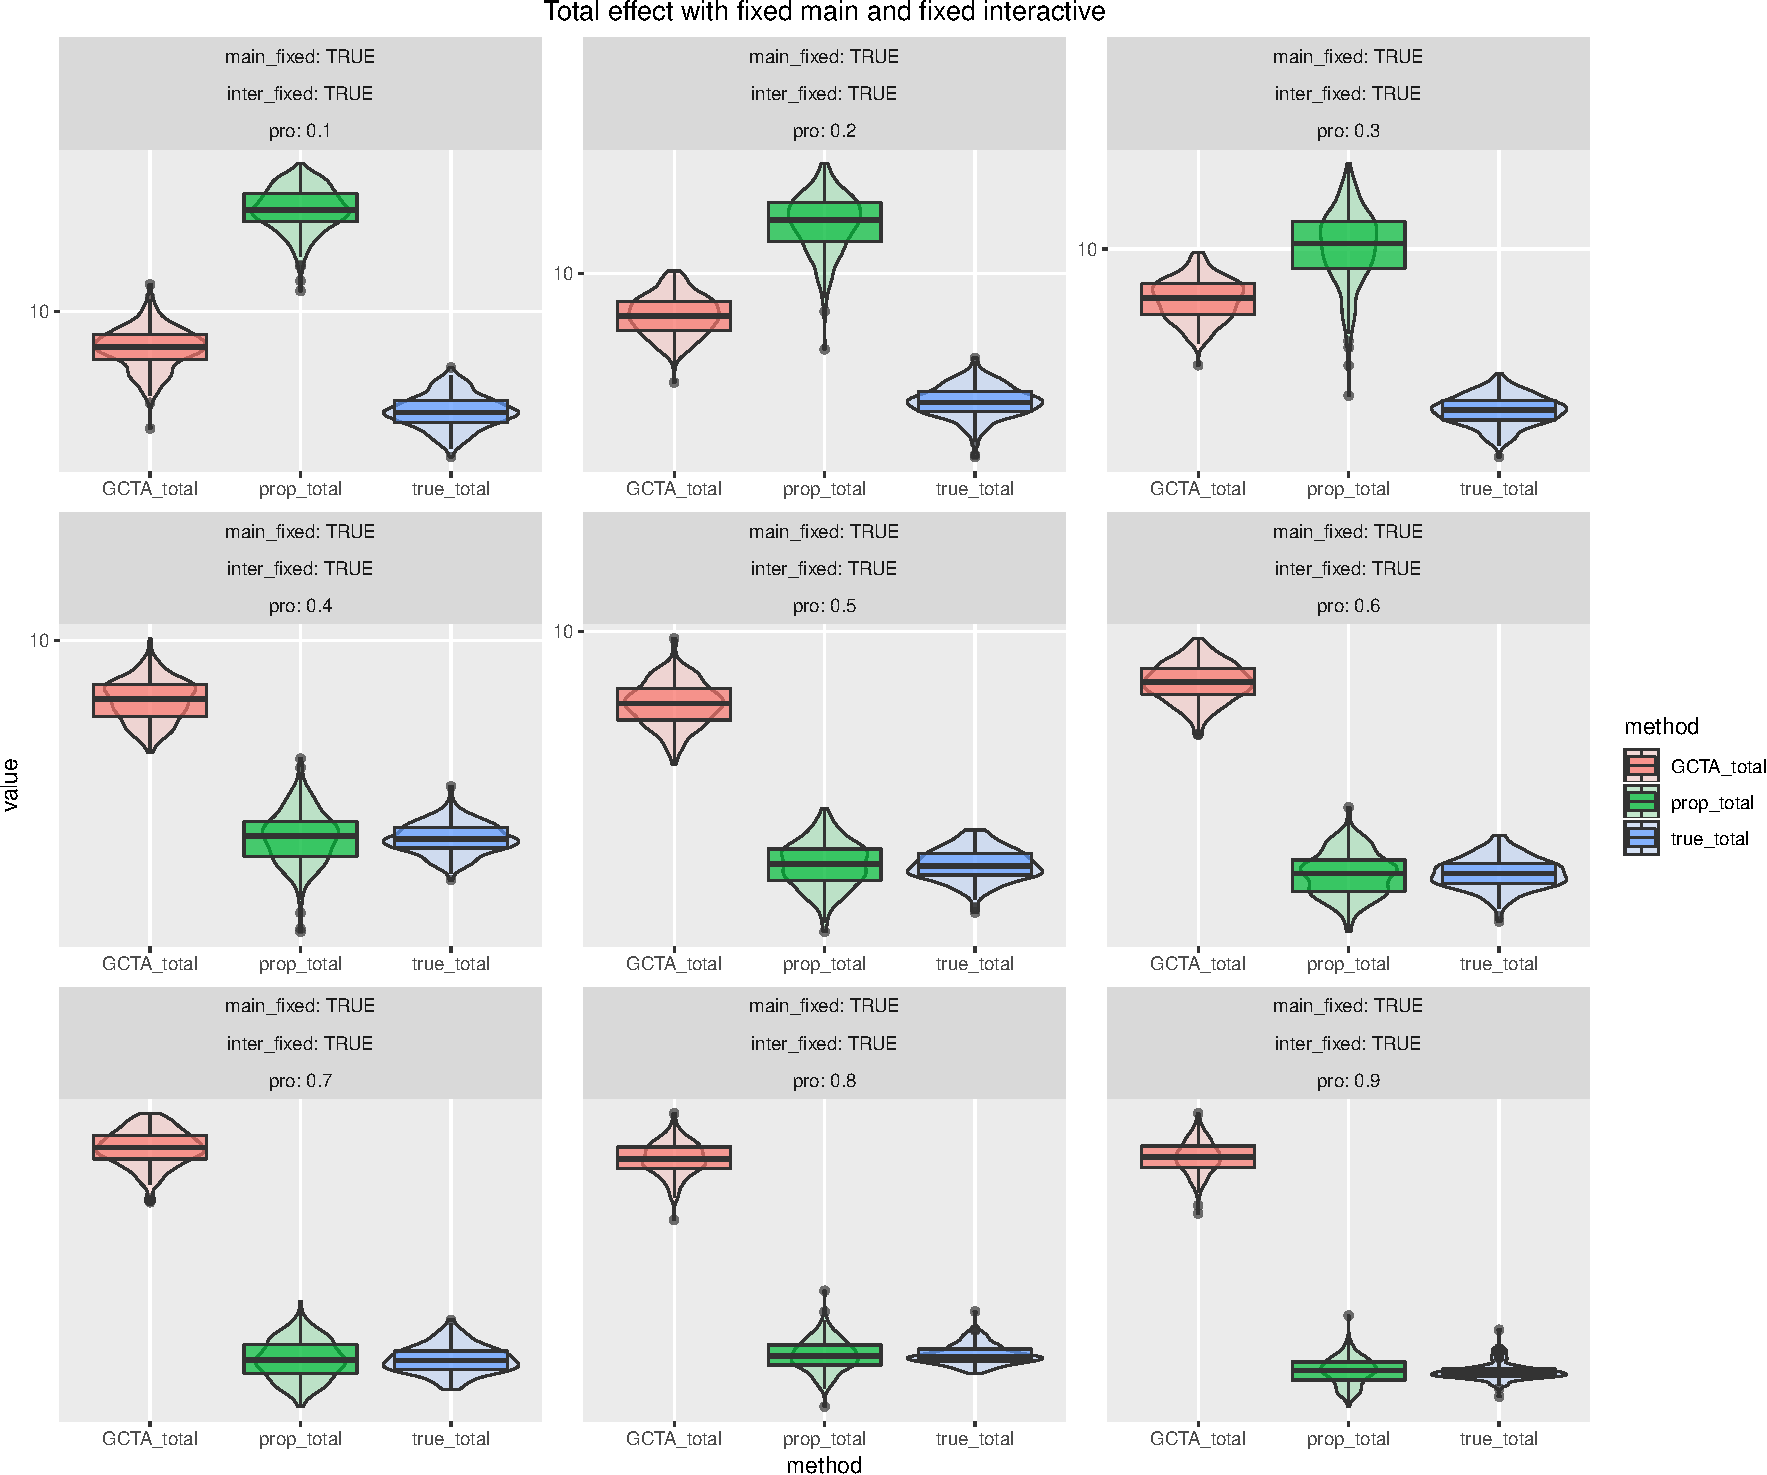
\includegraphics{Simulation_report_files/figure-latex/Total effect fixed fixed 33-1.pdf}
\caption{Total effect estimation with fixed main and fixed interaction}
\end{figure}

\begin{figure}
\centering
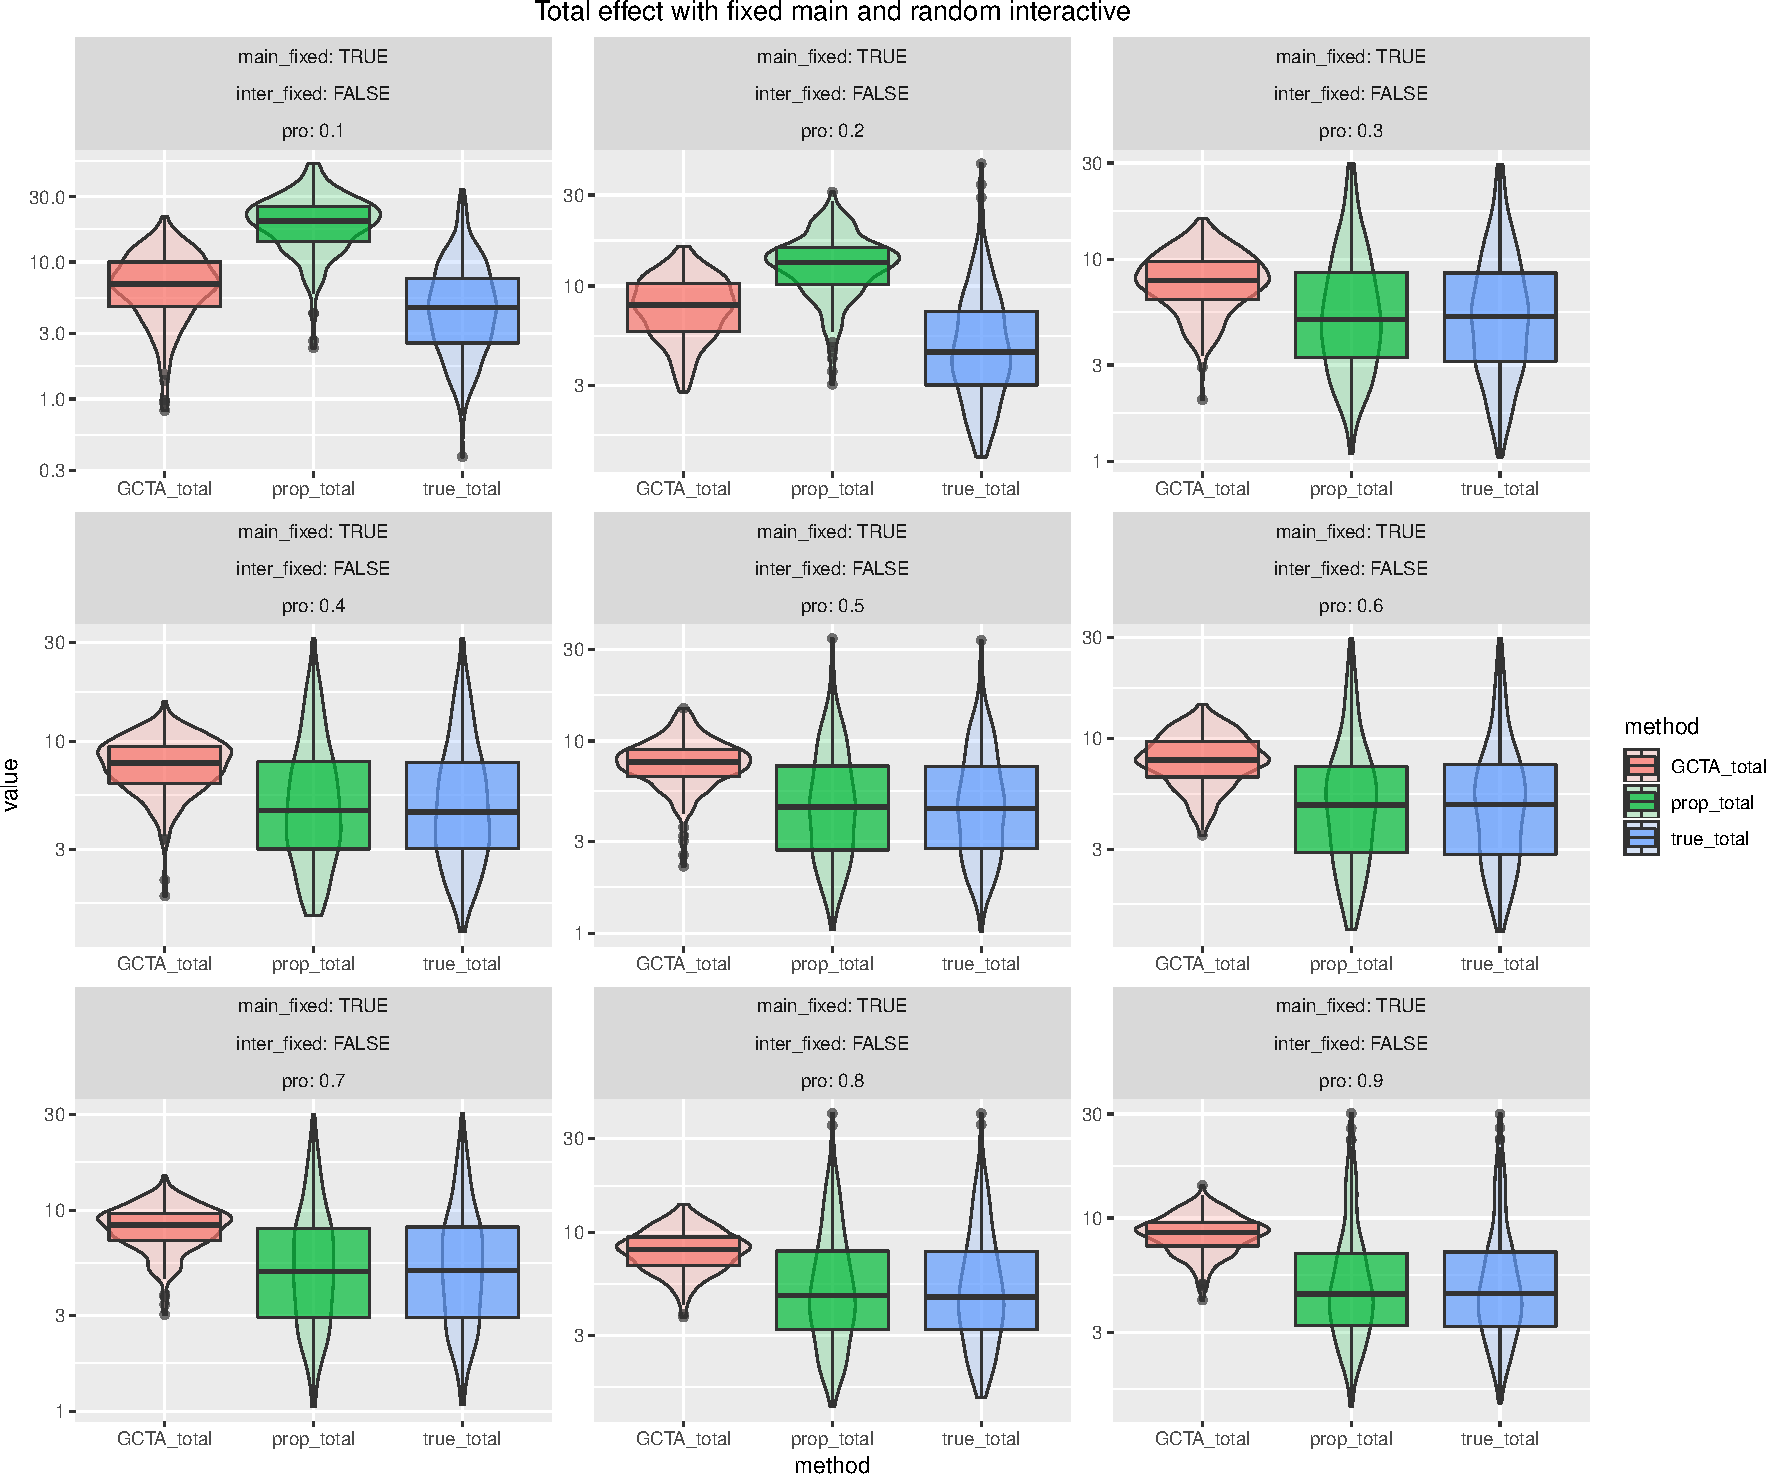
\includegraphics{Simulation_report_files/figure-latex/Total effect fixed random 33-1.pdf}
\caption{Total effect estimation with fixed main and random interaction}
\end{figure}

\begin{figure}
\centering
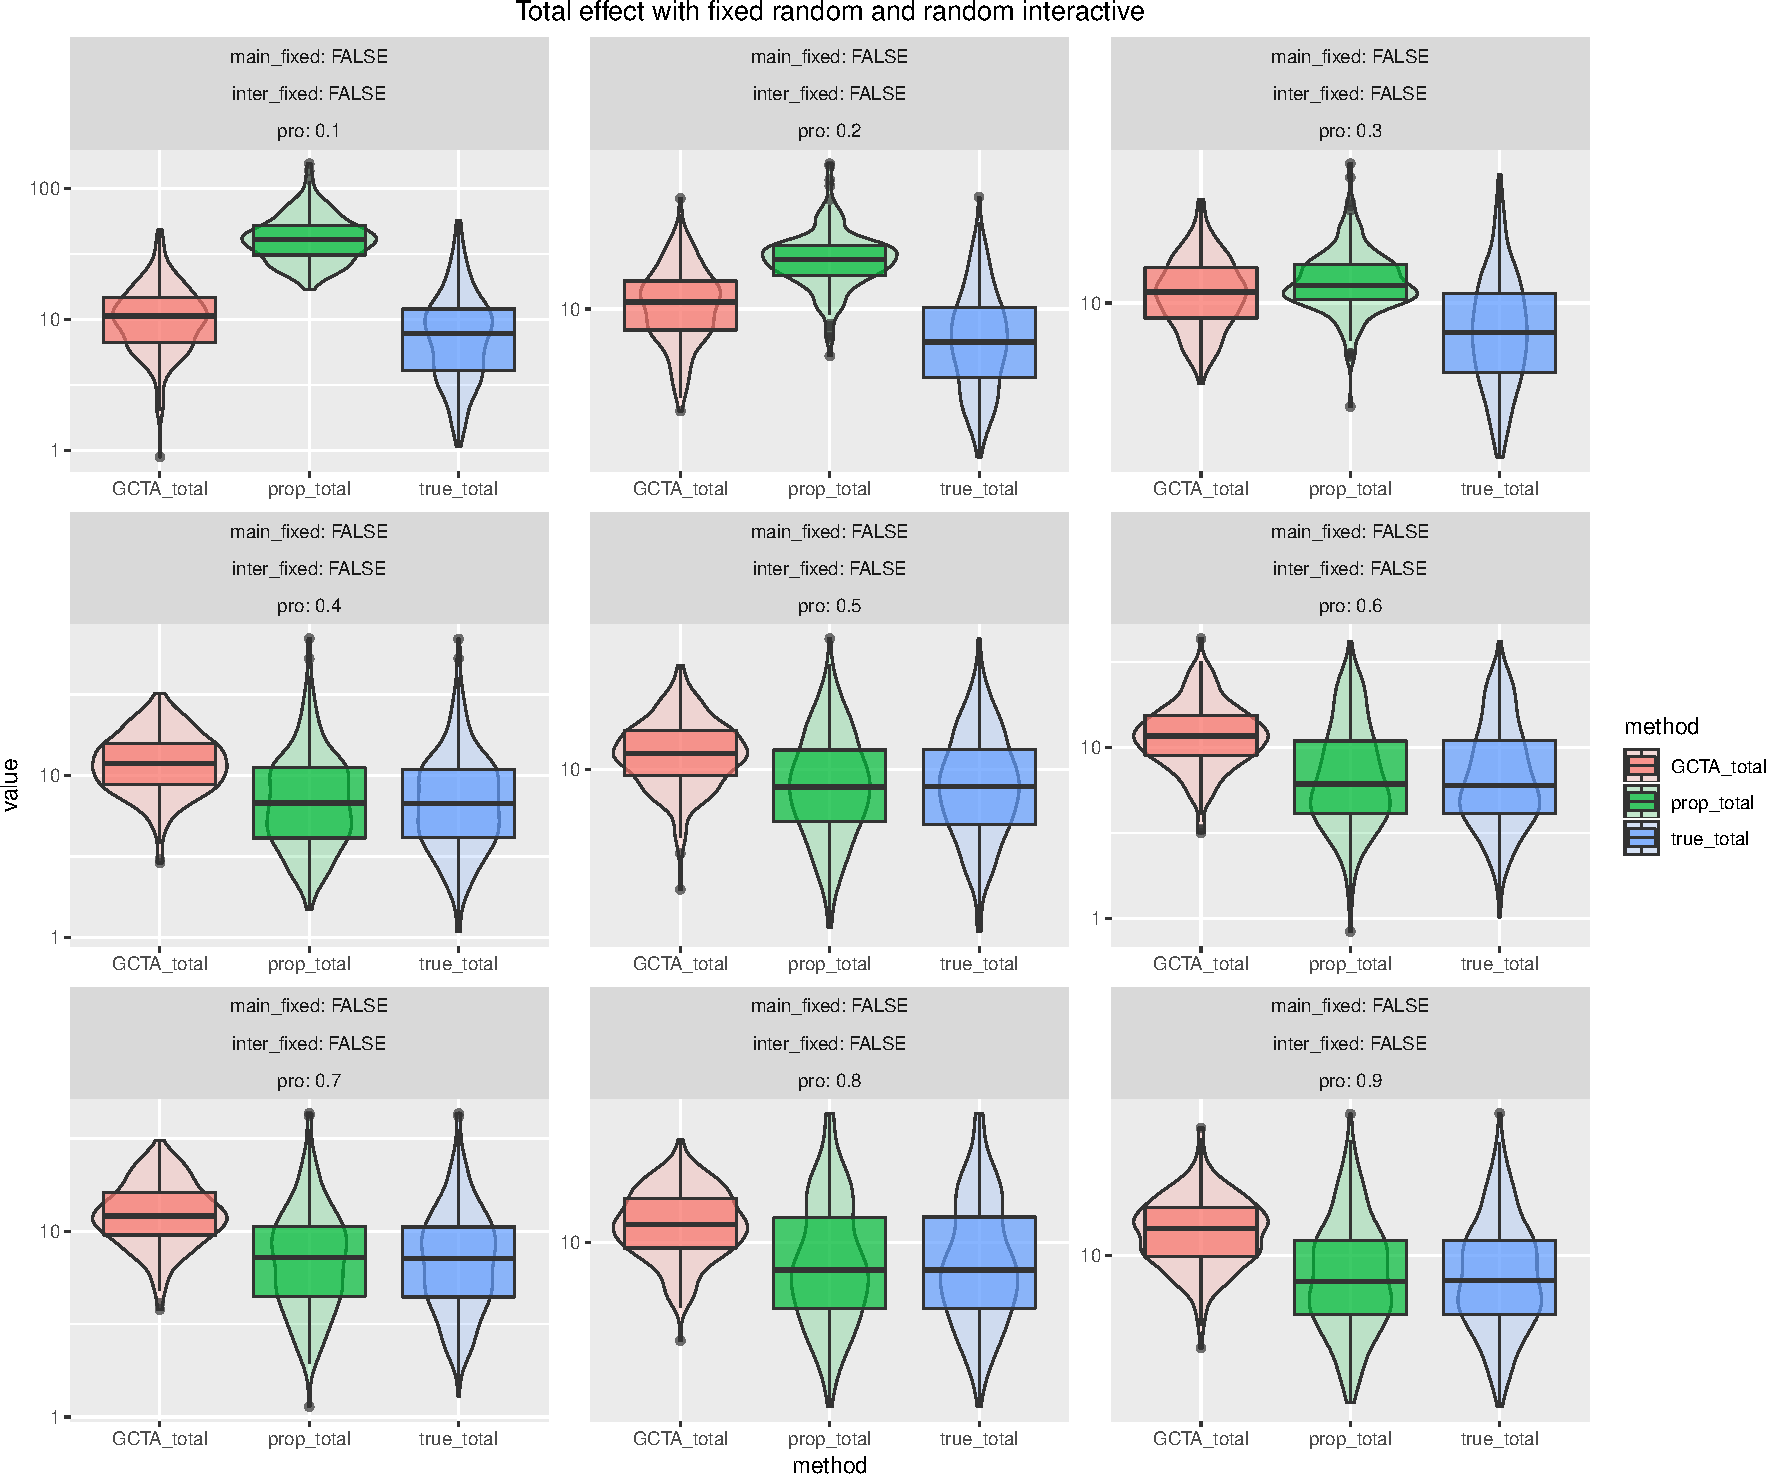
\includegraphics{Simulation_report_files/figure-latex/Total effect random random 33-1.pdf}
\caption{Total effect estimation with random main and random
interaction}
\end{figure}

\newpage 

\subsection{Main effect estimation (without interaction term in the
model)}\label{main-effect-estimation-without-interaction-term-in-the-model}

The purpose of this simulation is try to estimate the main effect only
given the true mode has interaction effect. Since we focus on the main
effect and ignore the interactive effect, the model we are using to do
the estimation is a wrong model.

\begin{figure}
\centering
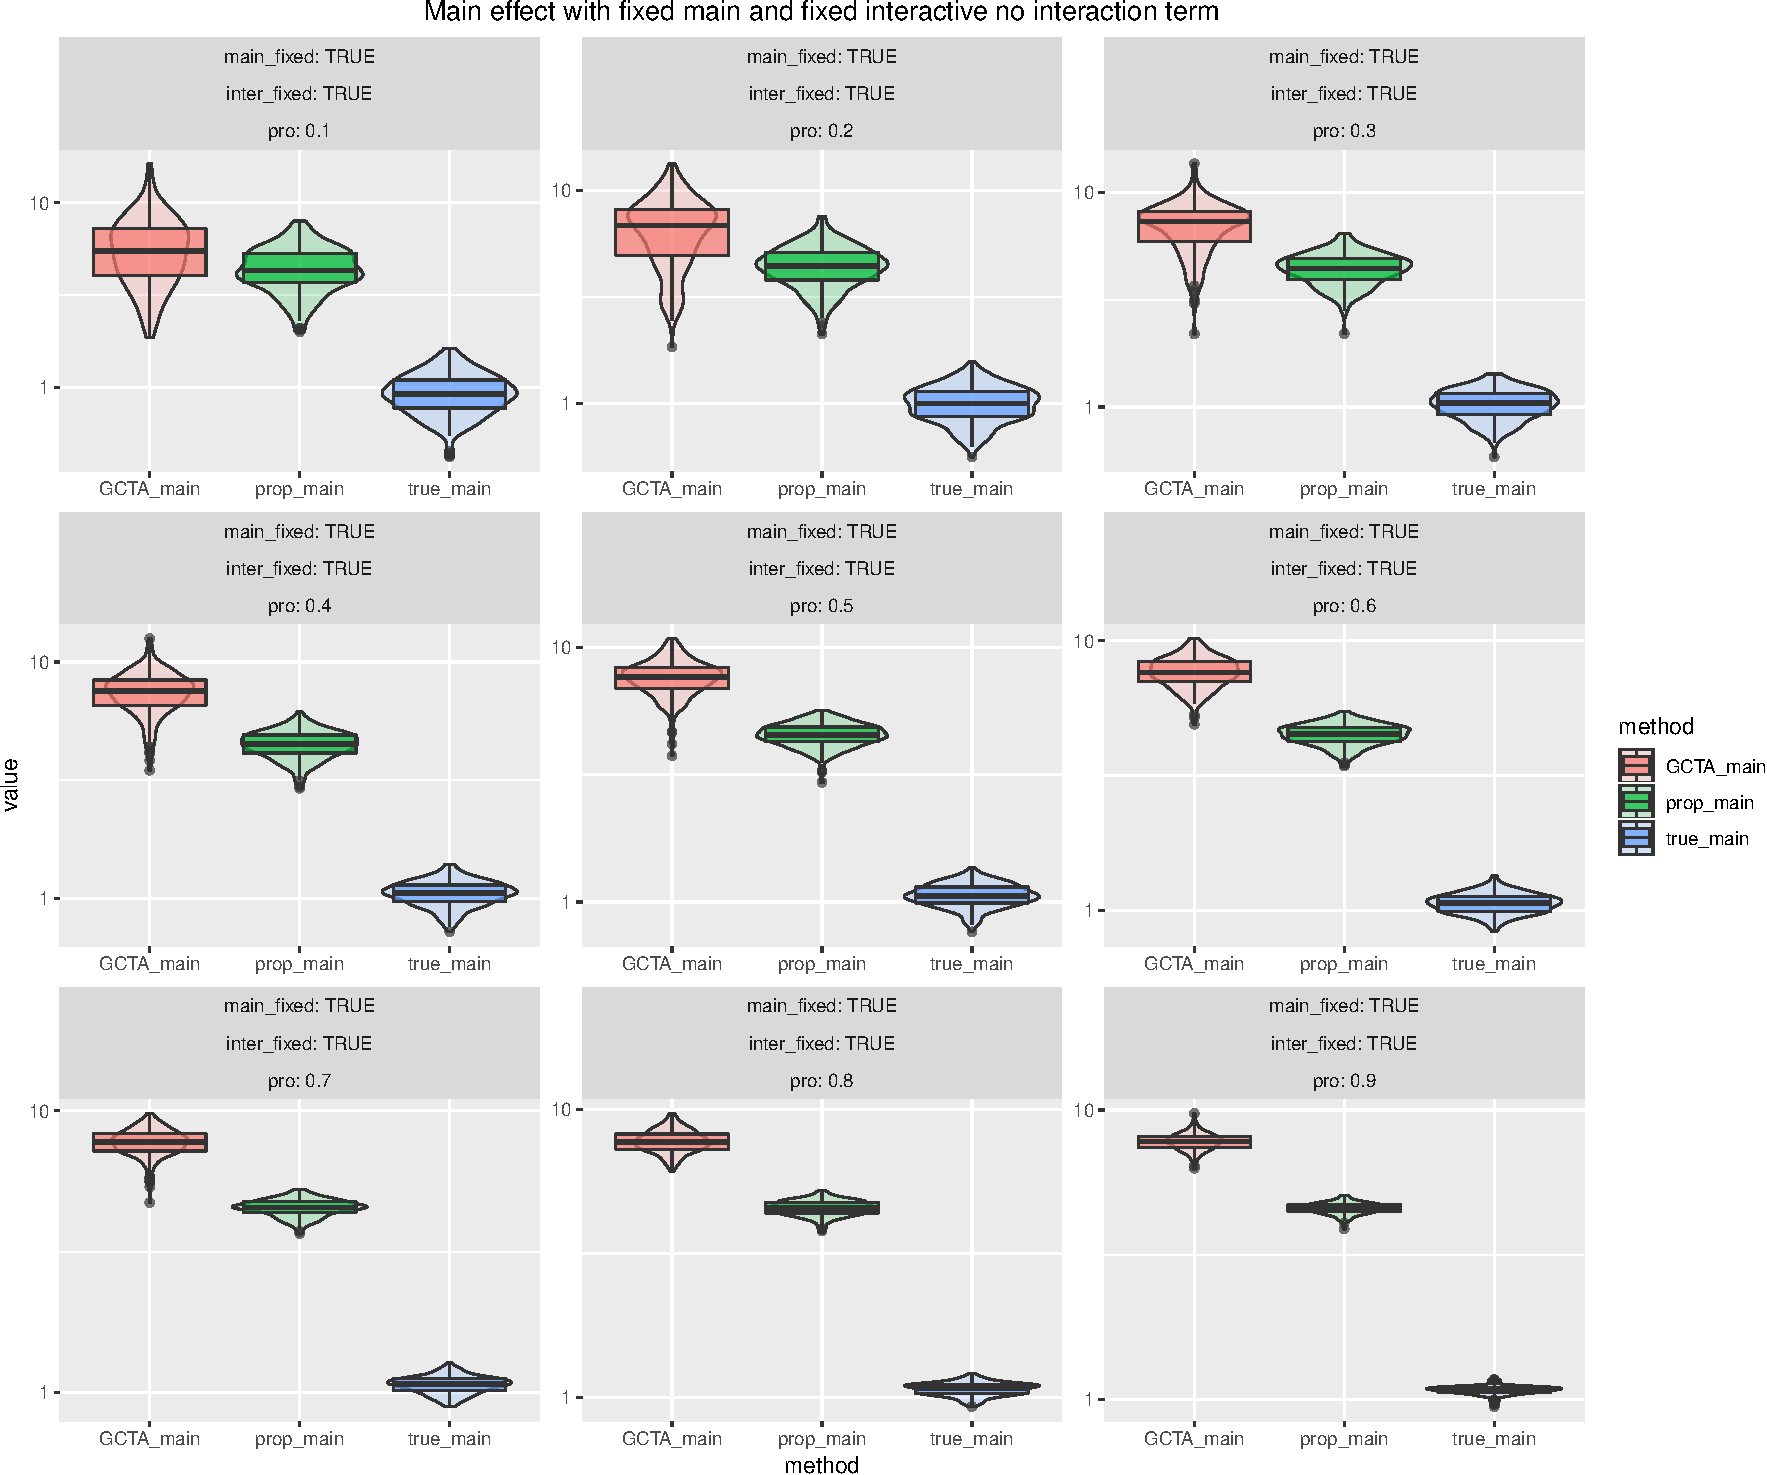
\includegraphics{Simulation_report_files/figure-latex/main effect fixed fixed without inter-1.pdf}
\caption{Main effect estimation with fixed main and fixed interaction}
\end{figure}

\begin{figure}
\centering
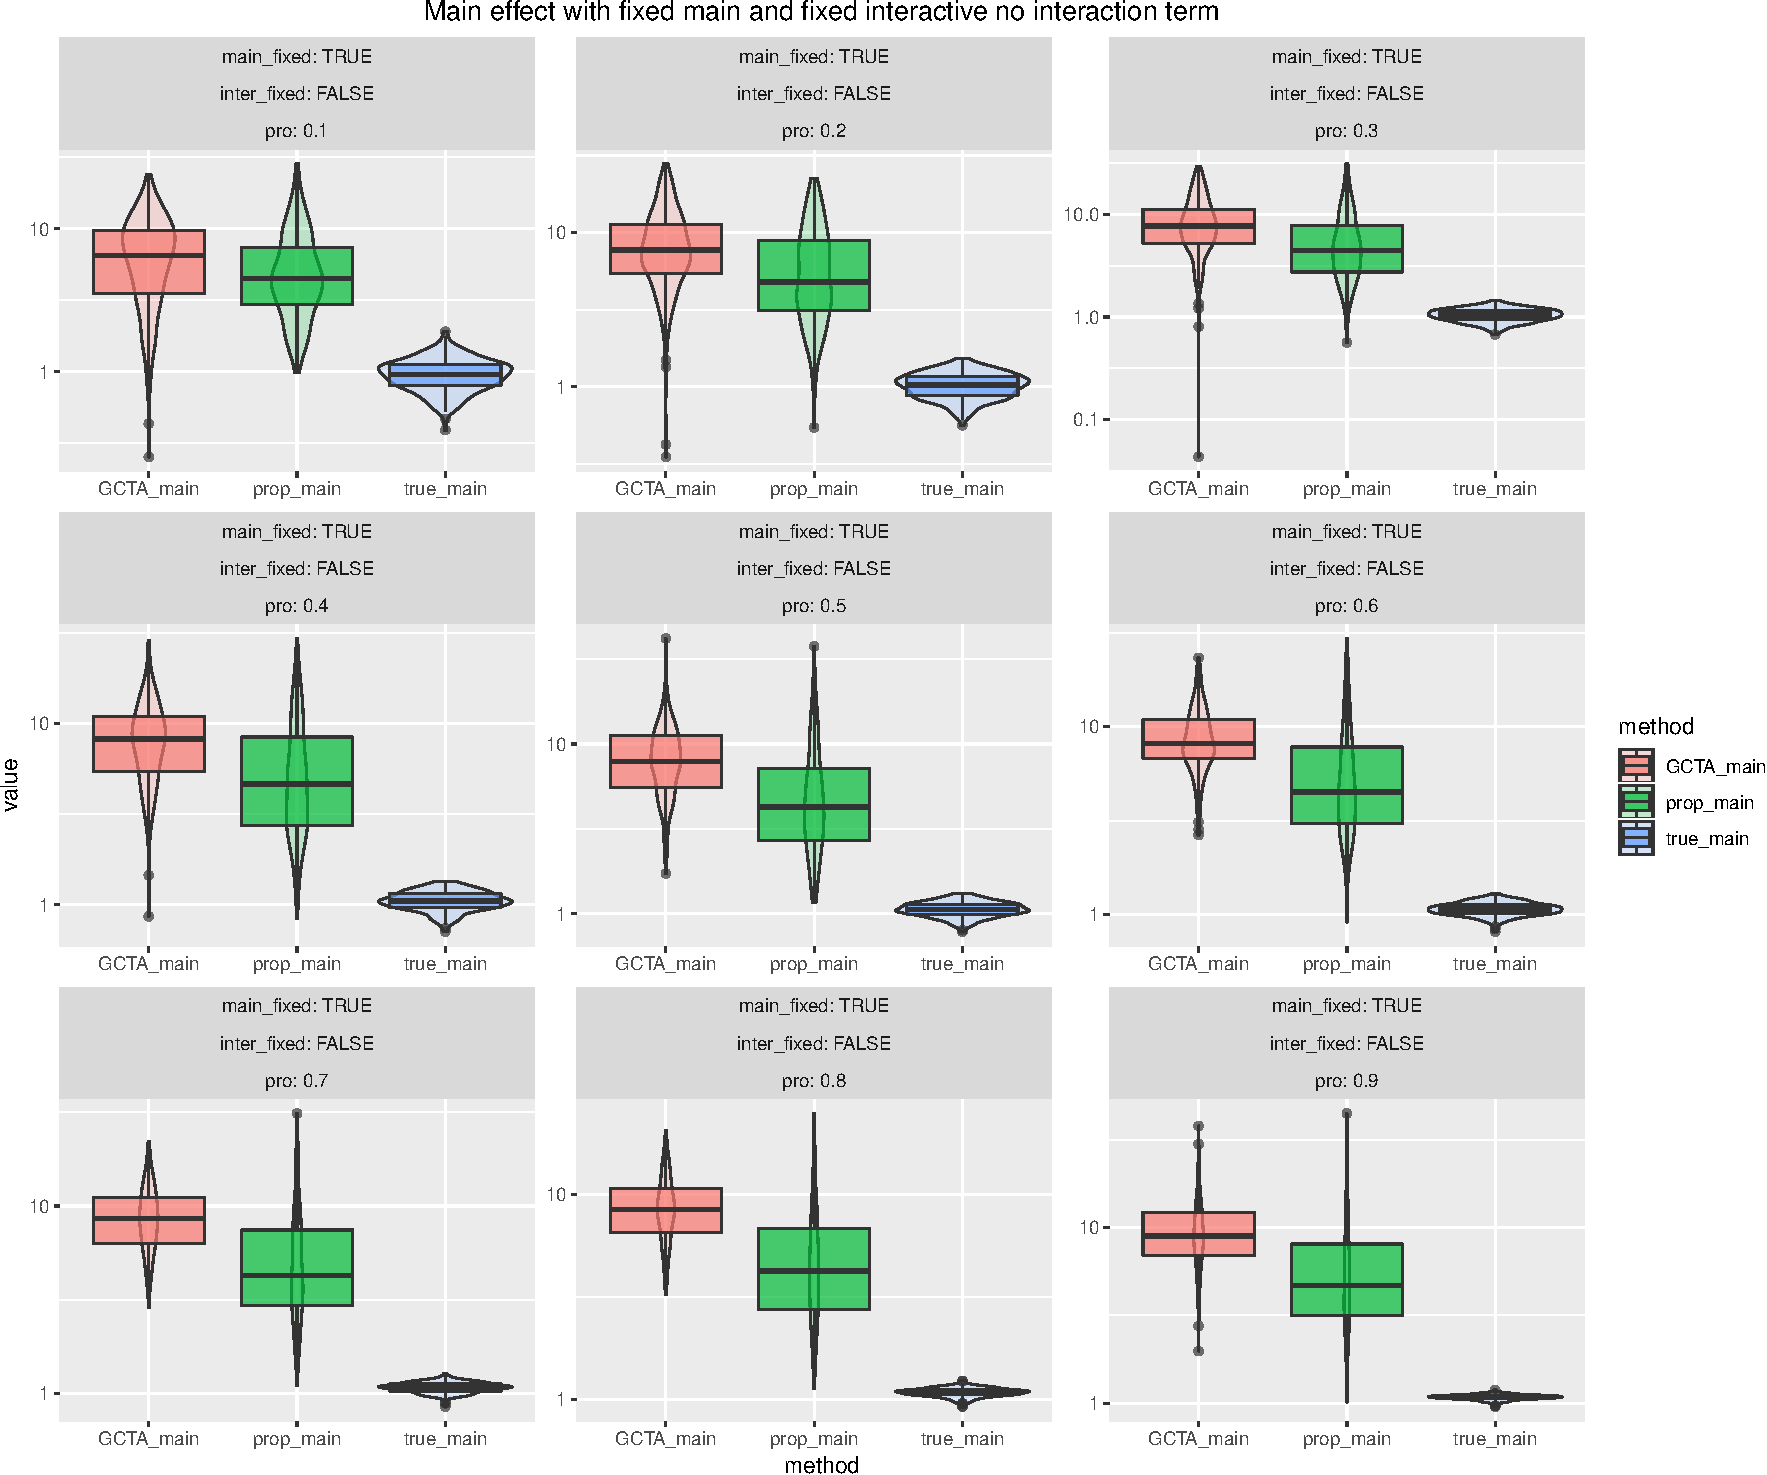
\includegraphics{Simulation_report_files/figure-latex/main effect fixed random without inter-1.pdf}
\caption{Main effect estimation with fixed main and random interaction}
\end{figure}

\begin{figure}
\centering
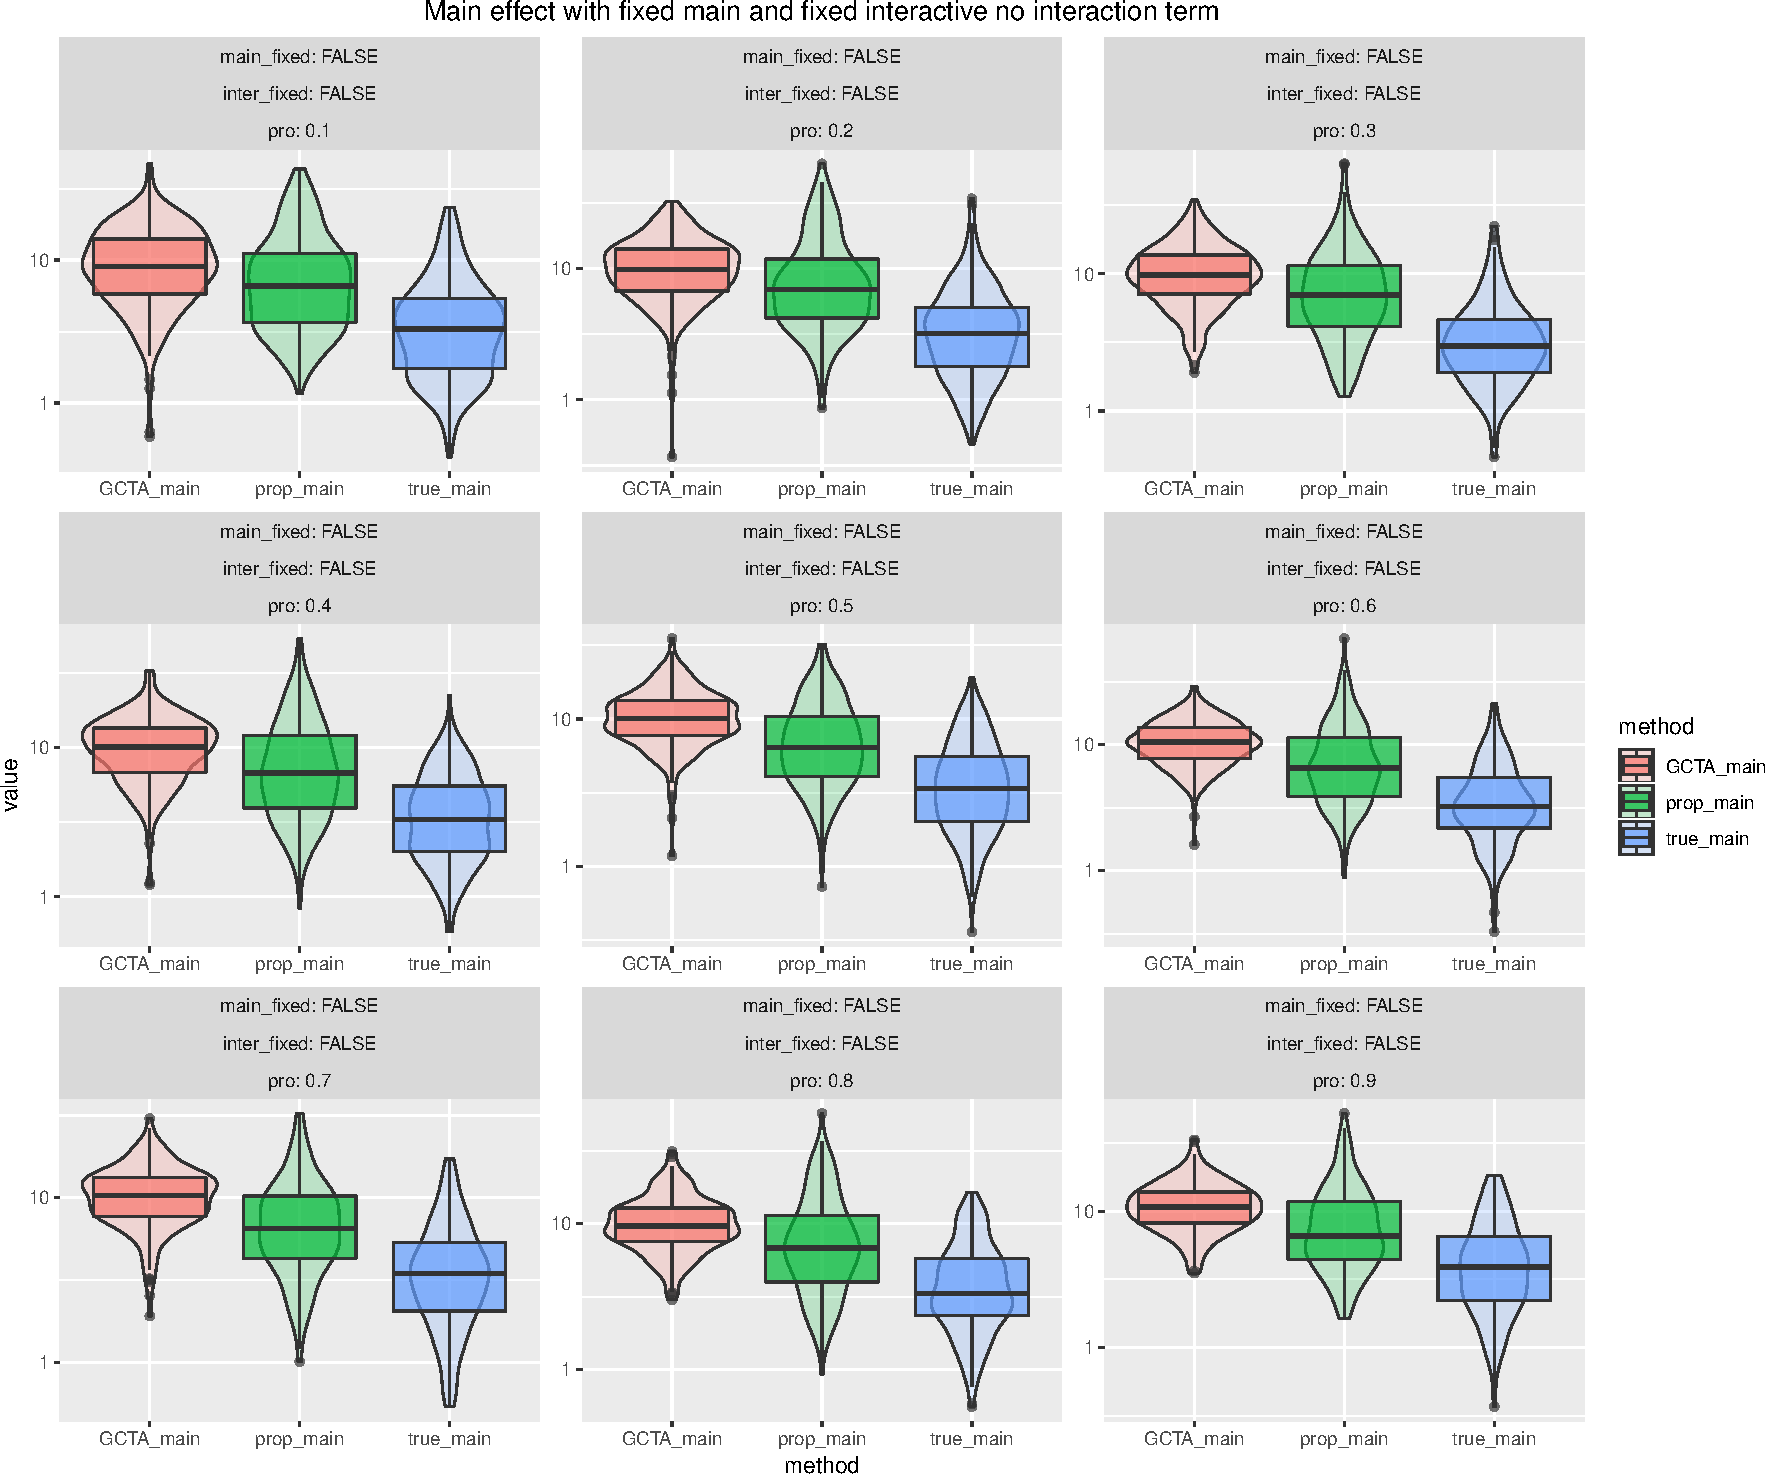
\includegraphics{Simulation_report_files/figure-latex/main effect random random without inter-1.pdf}
\caption{Main effect estimation with random main and random interaction}
\end{figure}

\newpage 

\subsection{Main effect estimation (with interaction term in the
model)}\label{main-effect-estimation-with-interaction-term-in-the-model}

\begin{figure}
\centering
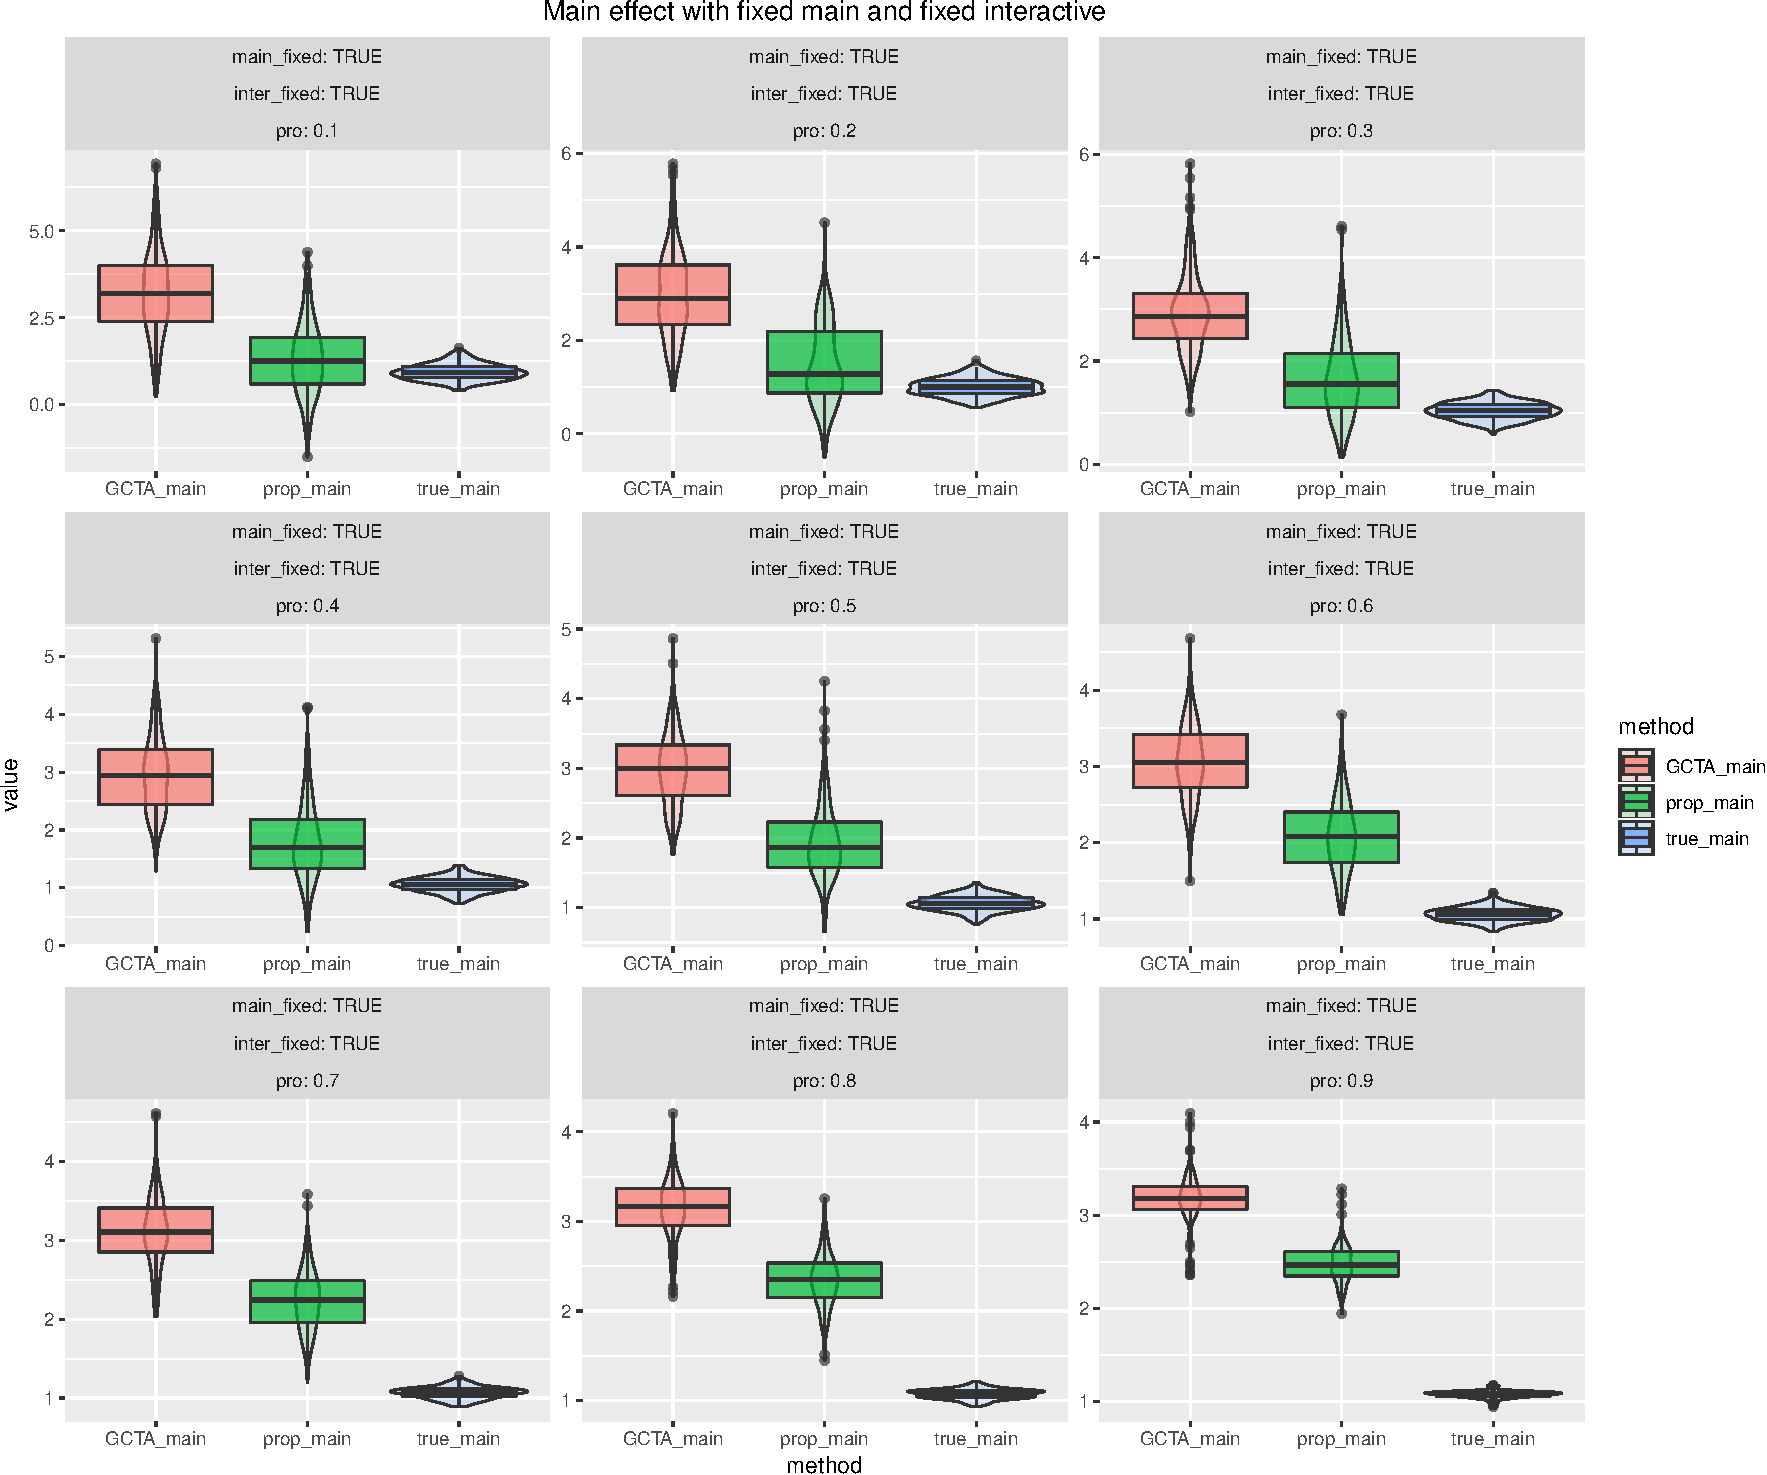
\includegraphics{Simulation_report_files/figure-latex/main effect fixed fixed-1.pdf}
\caption{Main effect estimation with fixed main and fixed interaction}
\end{figure}

\begin{figure}
\centering
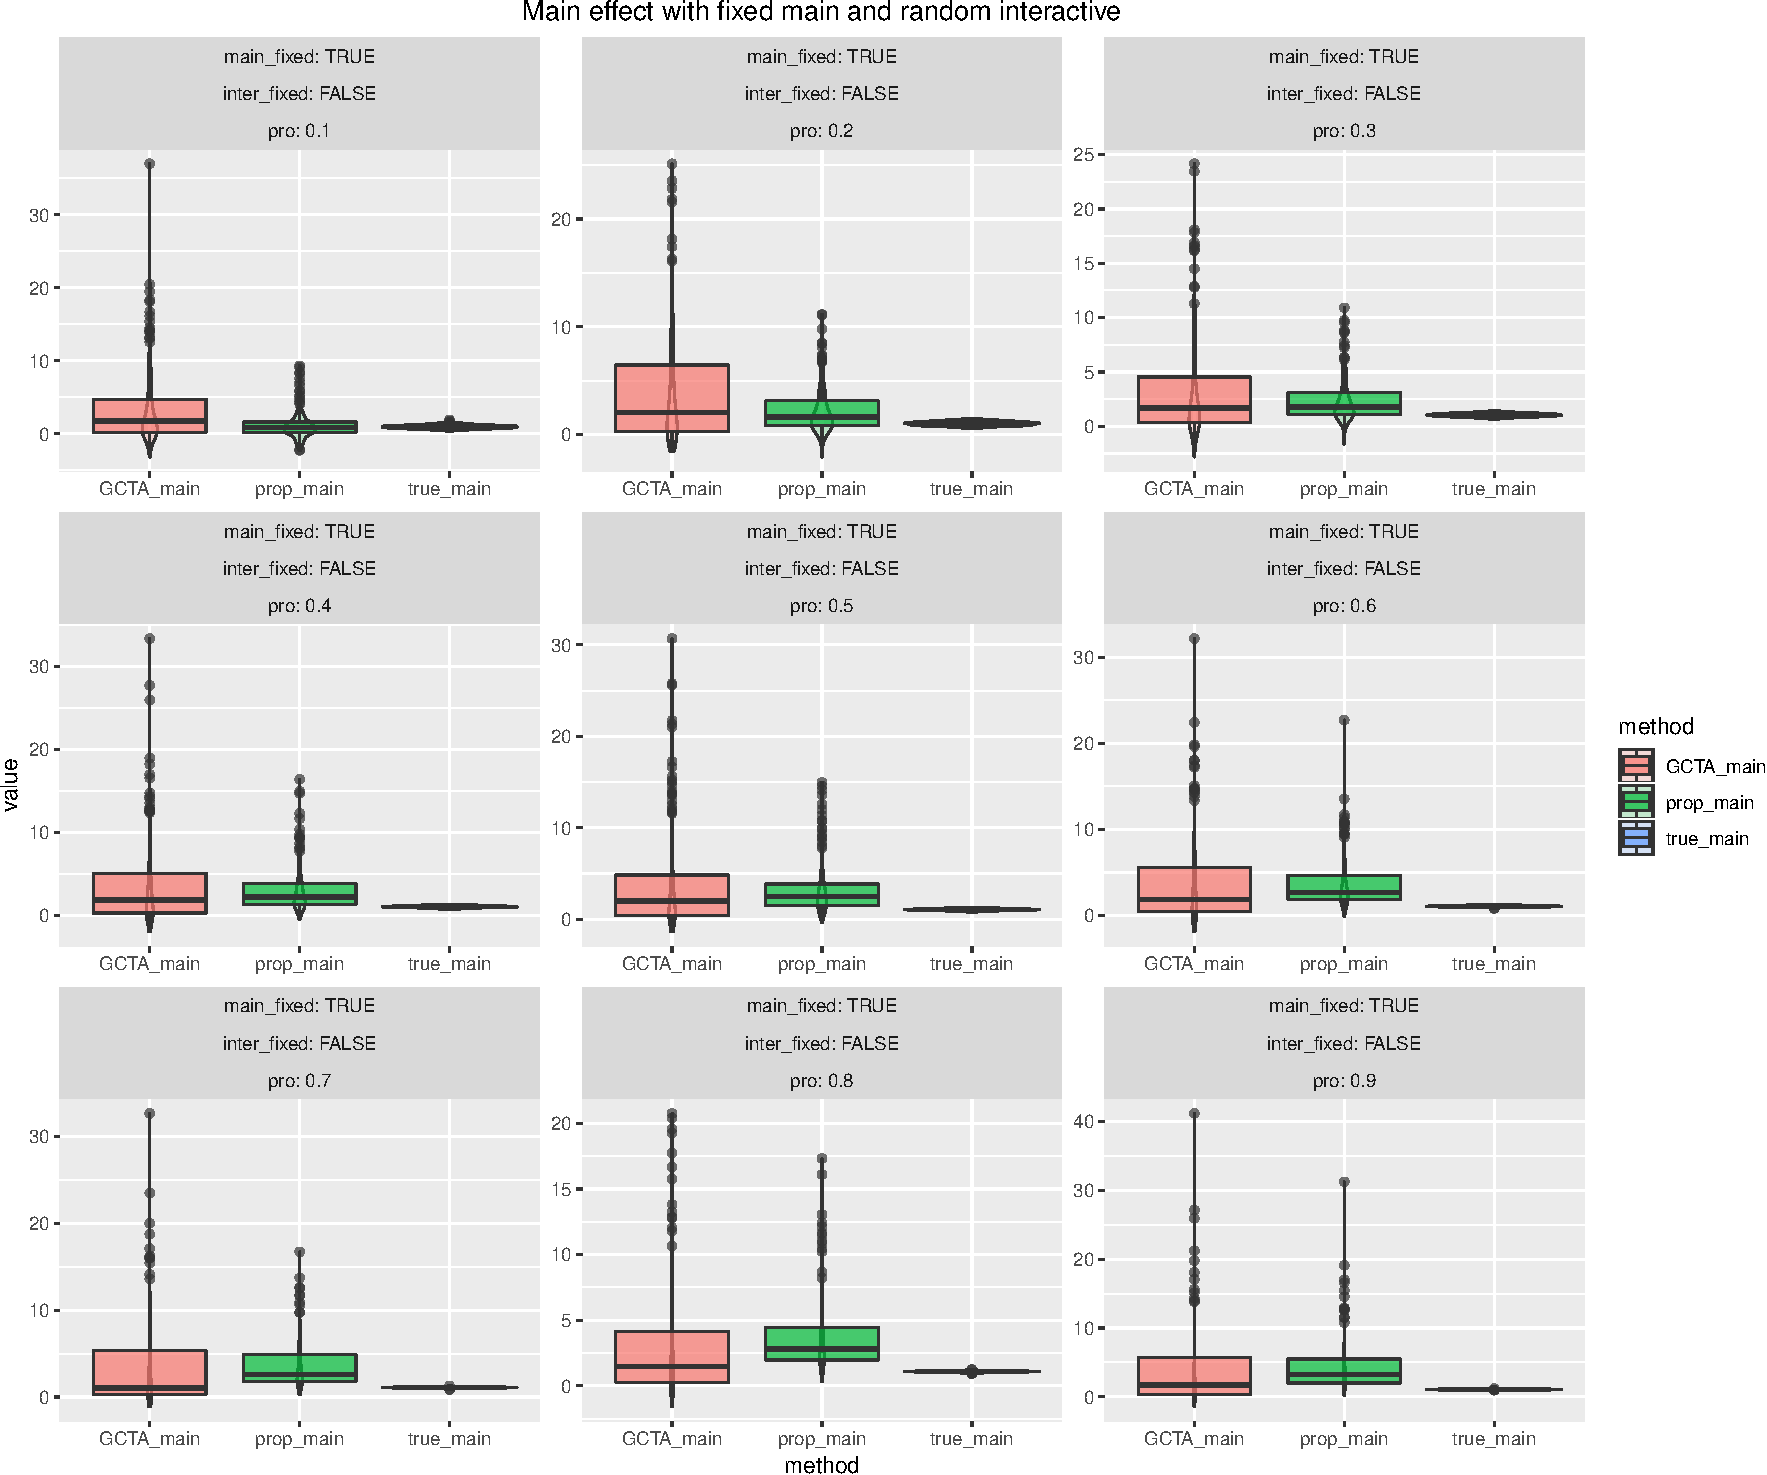
\includegraphics{Simulation_report_files/figure-latex/main effect fixed random-1.pdf}
\caption{Main effect estimation with fixed main and random interaction}
\end{figure}

\begin{figure}
\centering
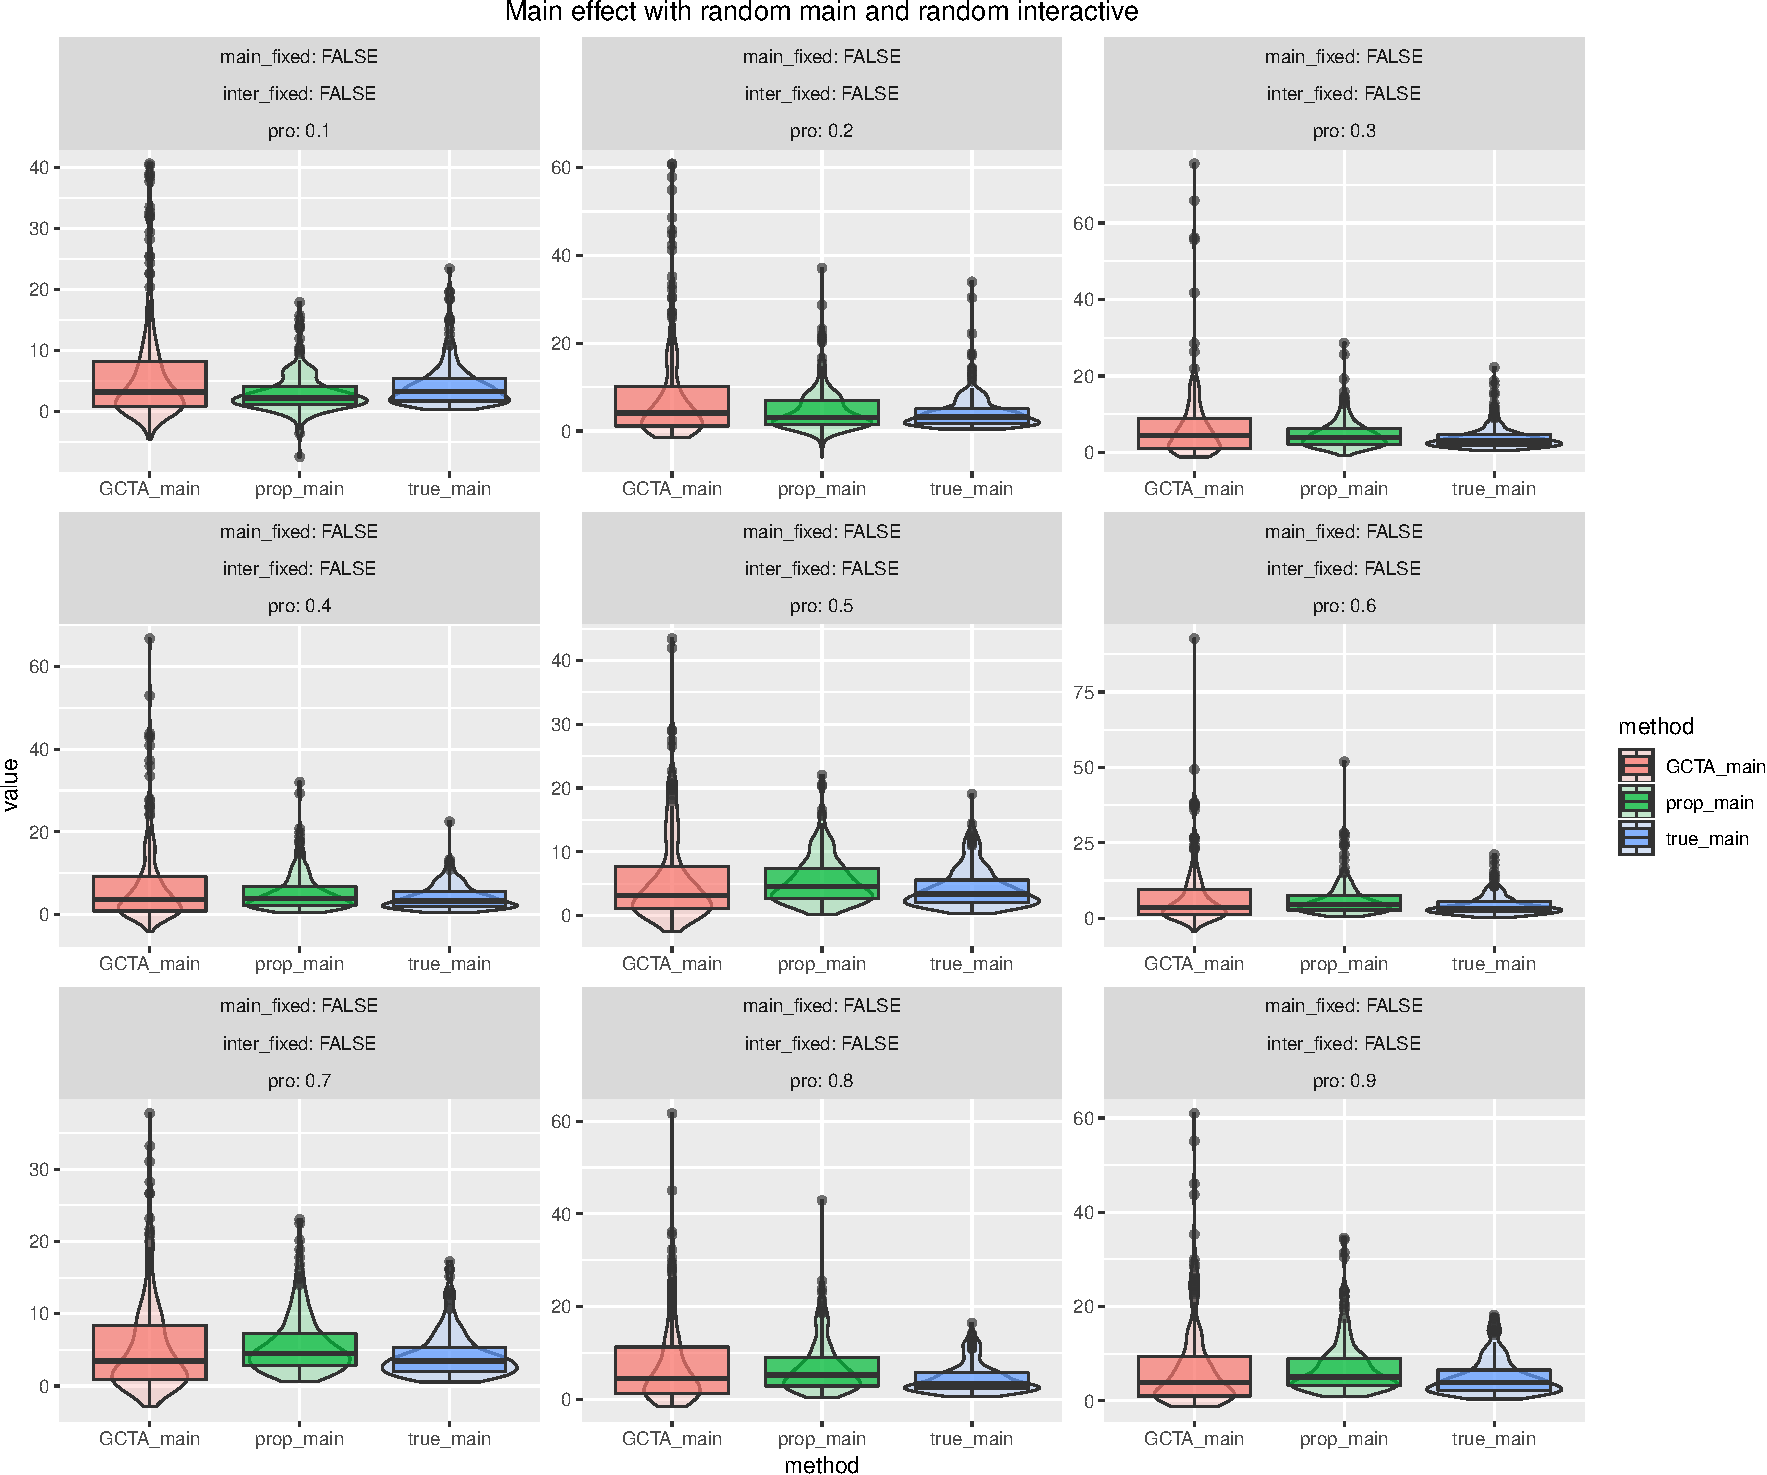
\includegraphics{Simulation_report_files/figure-latex/main effect random random-1.pdf}
\caption{Main effect estimation with random main and random interaction}
\end{figure}

\section{Conclusion}\label{conclusion}

\section{Further work}\label{further-work}


\end{document}
